\section*{Des îles et des espèces}\label{des-uxeeles-et-des-espuxe8ces}
\addcontentsline{toc}{section}{Des îles et des espèces}

\subsection*{En suivant Wallace,}\label{en-suivant-wallace}
\addcontentsline{toc}{subsection}{En suivant Wallace,}

Dans l'introduction de son livre ``Island Life'' paru en 1881, le
célèbre naturaliste Alfred Russel Wallace nous rapporte deux faits
étonnant qui justifient pleinement l'examen attentif de la répartition
géographique des espèces (Wallace, 1881). Premièrement, la biogéorphe
montre avec des exemples multiples que l'éloignemnet de deux régions du
monde n'est pas suffiant pour conclure quand à l'éloignement de leur
composition faunistique et floristique. Ainsi, comparer les groupes
d'oiseaux de l'île japonnaise d'Hokkaido avec ceux de l'Angleterre,
pourtant séparés par des miliers de kilomètres, révèle une proximité des
paysages ornithologiques bien supérieure à celle constatée entre les
îles indonesiennes de Bali et de Lombok distantes de quelques dizaines
de kilomètres seulement. Deuxièmement, en s'appuyant sur les différences
des faunes brésiliennes et africaines sous des latitudes similaires,
Wallace souligne la faiblesse du pouvoir prédictif des variables
climatiques pour décire les compositions fauniques. Par la mise en
évidence de ces deux éléments, Wallace souligne le besoin de croiser les
informations des distributions à la lumière d'une analyse taxonomique.
Dans le cadre de la théorie de l'évolution\footnote{Wallace a publié en
  1858 un article \emph{On the Tendency of Varieties to Depart
  Indefinitely From the Original Type} qui témoigne très clairement que
  ses idées sur les varitions temporelles des espèces étaient très
  proche de celle de Charles Robert Darwin a qui il avait d'ailleurs
  envoyé le manuscipt (Wallace, 1858).}, encore toute jeune en 1881,
cette analyse taxonomique est en fait une analyse historique. Wallace
affirme ainsi que la compréhension d'un problème spatial, celui des
aires de répartition de groupes d'espèces proches, n'est possible que
par une compréhension temporelle, celle de l'histoire des espèces, cette
idée est clairemnt énoncée dans la même introduciton :

\begin{quote}
« Many years study of this class of subjects has convinced me that there
is no short abd easy method of dealing with them; because they are, in
their very nature, the visible outcome and residual product of the whole
past history of the earth. »
\end{quote}

Tout au long de son livre, Wallace démontre que la connaissance à
l'échelle mondiale de la distribution des êtres vivants à travers le
monde permet de relier les différentes îles aux grands ensembles
régionnaux biologiques (que nous appelons aujourd'hui écozones) et que
ces groupes sont aussi relié par des liens historiques dont la taxonomie
révèle les traces. Ce travail de charactérisation d'ensemble
géographique conduit Wallace, dans un article de 1860 (Wallace, 1860), à
tracer la ligne séparant l'écozone indomalaise de l'écozone australienne
(qui sépare notamment Bali et Lomonk citées plus haut) qui porte encore
aujourd'hui son nom. L'éclaircissement de la géographie par l'histoire
est saississant et les exemples de Wallace sont autant de poids données
à la théorie de l'évolution. Le discours de Wallac porte sur des
processus à des échelles spataile et temporelles très grandes,\footnote{L'âge
  de la terre est très débattu à l'époque bien que de nombreux s'accore
  que les 6000 ans biblique sont insuffisant, Wallace avance,
  audacieusemnt, l'age de 500 milians d'année.} et bien que
l'éclaircissement substantiel des répartitions géogrpahiques des êtres
vivants par l'évolution, cette expliqcation se double d'un obstacle
épistémologique important : si l'explication ultime de la présence d'une
espèce en un point donné est le produit d'une série de contingences
historiques, sur quoi bâtir une théorie de la biogéographie? Ce n'est
qu'au XX\^{}ème siècle que des réponses convaincaites émergeront avec a
fructuseuse rencontre du mathématicien et biologiste Robert Helmer
MacArthur et du myrmécologue Edward Osborne Wilson.\footnote{Cet actuel
  professeur émérite à l'université d'Harvard est reconnu pour ces
  apport en biologie et en sociologue, il est l'auteur de 32 livres mais
  c'est pour son immense connaissance des fourmis que j'ai choisi
  l'adjectif de myrmécologue.}

\subsection*{En suivant MacArthur et
Wilson}\label{en-suivant-macarthur-et-wilson}
\addcontentsline{toc}{subsection}{En suivant MacArthur et Wilson}

La collaboration de ces deux jeunes biologistes a mené à la formulation
d'une théorie de la biogéographie insulaire publiée en 1967 sur laquelle
je reviendrai abondammnent tout au long de mon introduction (MacArthur
and Wilson, 1967) puisqu'elle est un des piliers de ma thèse. Leur
démarche a été de collecter un grand nombres de données sur différents
groupe d'espèces sur des îles dispersées un peu partout dans le monde et
pour essayer de mettre une cohérence à travers ces faits avec un cadre
théorique puissant. Comme indiqué au au dernier chapitre de leur livre
de 1967, ces auteurs souhaite voir la biogéographie entrer dans une
nouvelle phase :

\begin{quote}
« Biogeography has long remained in a natural history phase,
accumulating information about the distribution of species and higher
taxa and the taxonomic composition of biotas. Interpretative reasoning
has been largely directed to the solution of special problems connected
with the histories of individuals taxa and biotas. Without doubt this
descriptive activity will continue to be of fundamental importance to
the science, one of the most physically adventurous of all scientific
entreprises and, in the richness of the detail it unfolds, esthetically
pleasing. But biogeography is also in a position to enter an equally
interesting experimental and thereotical phase. »
\end{quote}

MacArthur et Wilson affirment que l'étude de la distribution des espèces
doit sortir du royaumes des contingences pour devenir un objet de
science au sens d'être manipulé aussi bien expérimentalement que par
l'abstraction mathématique. La validation expérimentale de la théorie a
été menée par Wilson et son étudiant au doctorat de l'époque, devenu
depuis le grand écologue Daniel Simberloff, avec une expérience de
défaunation de six petits îlots de mangrove dans la Baie de Floride
(Daniel S Simberloff and Edward O Wilson, 1969). La travail
d'abstraction mathématique a été conduit par MacArthur dans le livre de
1967 et prolongé dans les annexes de son livre de 1972 (MacArthur,
1972). Leurs efforts conjugués ont donné le jour à une vision puissante
de la biogéographie dans laquelle la richesse spécifique d'une île
donnée est le résultat de deux porcessus oposés : un processus de
colonisation qui augmente le nombre d'espèce sur l'île et un porcessus
d'extinction qui le diminue. En reliant ces processus aux propriétés
physiques de l'île (aire et isolation) et en interprétant la richesse
spécifique des îles en terme d'équilibre entre ces deux processus, les
auteurs parviennent à expliquer de manière convaincante les relations
observées entre richesse spécifique, taille de l'île et isolement (je
reviens amplement sur cette théorie dans le troisième temps de cette
introduction).

Le paradigme données par les auteurs est un lègue qui a eu un impact
considérable sur les développemnt théorique en écologie
({\textbf{???}}). Au coeur de la réussite du modèle, il y a la vonlonté
de mettre l'espèce au coeur de la biogéographie de ne pas simplemnt
parler de grands ensembles régionaux et d'em discuter l'histoire nais
aussi de coprendre les mécanismes biologiques plus fins qui sont le
moteur essentiel de la variation dans la distribution des espèces. Tout
l'intérêt de leur \emph{biogéographie de l'espèce} (terme donné à
l'avant-dernière phrase de leur livre de 1967) est dans l'affirmation
qu'il faut repgarder les contraintes conjointe de l'évolution (qui met
un certain nombre de groupes taxonomiques en présence) et du context
écologique qui régit les conditions d'extinction. Cette intrication de
l'écologie et de l'évolution est bien inscript dans la pensée de
MacArthur et Wilson même si la puissance de leur vision réside dans le
fait de les occulter en partie.

Près de 50 and après la parution de leur livre, une des clef en biologie
semble être la compréhesion des retro actions l'écologie et de
l'évoluton dans les varitions spatiale et temporelles de la
biodiversité. On peut reprendre les trois aphorismes cités par Schoener
(2011a) :

\begin{quote}
« Nothing in biology makes sense except in the light of evolution. »
(Dobzhansky, 1964)
\end{quote}

\begin{quote}
« This was supplanted half a century later by (2): Nothing in
evolutionary biology makes sense except in the light of ecology. »
(Grant and Grant, 2008)
\end{quote}

\begin{quote}
« Nothing in evolution or ecology makes sense except in the light of the
other. » (Pelltier, 2009)
\end{quote}

Au sein de la communauté, l'idée qu'il est difficle d'isoler les deux
discipline et cela indépendamment de l'échelle cnsidérée semble gagner
du terrain. Un parrallèle avec les sciences humaines me semble possible
l'écologie serait à la biologie ce que la géographie est aux sciences
humaines et aussi que l'évolution serait à la biologie ce que l'histoire
est aux sciences humaines. Nous pouvons bien sur étudier l'une sans
l'autre, mais le dialogue entre les deux disciplines est indispensable
sinon elles avancent en faisant des hypothèses fortes sur l'autre et qui
finiront éventuellement par nuire à la compréhension. Aisin supposé que
les ressort de la varation sont puremnt des mécanimes écologique alros
que dans certains système la variation allélique peut affecter
rapidement et formtement la démogrpahie est problématqie (Pelletier et
al., 2007). Néanmoins chaque discipline a des connaissance à apporter
pour nourir ce dialogue et la Biogéogrpahie est le champ qui tente de
conprendre l'information refermée dans les distributions d'espèces.

\subsection*{Quelles informations renferment les distributions
d'espèces?}\label{quelles-informations-renferment-les-distributions-despuxe8ces}
\addcontentsline{toc}{subsection}{Quelles informations renferment les
distributions d'espèces?}

Cette question est non seulement une invitation à découvrir les raisons
de la présence de tel ou tel organisme en un lieu donné du globe, mais
elle suggère ausi que certaines informations ne sont pas obtenue par
l'analyse de répartion géographique des espèces. Les grands auteurs
mentionnés dans les paragraphes précédents y ont apporté des éléments de
réponse essentiels : Wallace a montré que la distribution reflètait en
partie les liens de parenté entre les esèces, quant à MacArthur et
Wilson, ils ont suggérés que ces distributions étaient le résultats de
processus écologiques dynamiques. Examiner les aires de répartition,
relever les variations spatiales et temporelles, mais aussi détailler la
géométrie exacte au regad de variables abiotique ou à la lumière de la
géométrie d'autres espèces est une clief pour apprécier les mécanismes
sous-jacents.

Dans son ouvrage de 1972, MacArthur se livre à un examen approfondi du
sujet en examinant des aires de répartition au regard des variables
climatiques mais aussi les variations teporelles ou encore les relations
qu'il existe entre les distributions d'espèce en compétition. Il propose
un cadre mathématique pour comprendre l'impact de la prédation et de la
compétition sur lequel repose un prinicpe de ségrégation spatiale
d'espèce en compétition : deux compétiteurs ne peuvent pas co-occurer
(être trouver au même endroit) sauf éventuellement sur zone très
restreinte de leur distribution (MacArthur, 1972). Toujours dans ce même
ouvrage, MacArthur évoque la distribution en damier
(\emph{checkerboard}) que peuvent générer des espèces en compétition. Ce
type de distribution sera approfondie et quantifiée par Jared Diamond
(Diamond, 1975) dont les travaux déclencheront un débat important sur la
determination de modèle null de co-occurrence (Connor and Simberloff,
1979).

L'analyse des distributions d'espèce est riche quand l'anaylse a de
multiple approche. Bien entendu dans un premier temps, l'examen sur de
multiple aires de répartition est un premier pas pour y déceler des
phénomènes répétés nécessaires à l'élaboration des théories (MacArthur,
1972). C'est aussi dans l'examen des variations spatiales et temporelles
que les informations abondent car si ces variations sont par exemple
reflétées dans els changelmnts climatiques, cela justifie l'espoir de
comprendre l'évolution des distributions d'espèces dans un context de
chanmgement climatique. De plus, l'examen d'une distribution est aussi à
faire par comparaison avec d'autre espèces notamment les espèces en
interaction pour voir si la biologie laisse ces empreintes dans la
géométrie de ces aires de répartition. C'est ainsi que dans ma thèse, je
propose de regarder l'intersection des aires d'un ensemble de proies
pour comprendre ce que la co-occurrrence peut nous apprendre.

\subsection*{Enjeux de la connaisssance de la répartition géographique
des
espèces}\label{enjeux-de-la-connaisssance-de-la-ruxe9partition-guxe9ographique-des-espuxe8ces}
\addcontentsline{toc}{subsection}{Enjeux de la connaisssance de la
répartition géographique des espèces}

Les enjeux fondamentaux ont été évoqués plus haut : les observations et
la compréhension des causes profondes de la géométrie et la dynamique
des aires de répartitions des espèces ont déjà amené à des découvertes
majeures en écologie et en évolution. La phase d'expérience et de
Théorie décite par MacArthur et Wilson se poursuit et l'espoint se
tourne vers la possibilité d'obtenir des prédictions fiabkes sur les
aires de répartitions futures d'une espèce données. Ce problème est
d'autant plus pesant dans la litérature en biogéograhique dans le
contexte actuel des changements globaux. En biogéogrpahie, les
changements climatiques ont canalisés l'attention et les chercheurs
constatent l'ampleur à laquelle la biodiversité mondiale est affectée
par ces derniers (Koh, 2004, Bellard et al. (2012)). Le volonté
d'anticiper où seront les espèces demain a également engendré un effort
de développemnet d'outils statistiques essentiellement centrés sur la
correlation entre les variables abiotiques et occurrence des espèces
(Elith et al., 2006).

En choississant de parler de telle ou telle espèce, nous glissons
rapidement à des enjeux sociaux et économiques évidents. Ainsi, pour un
pays comme la France, comprendre les impacts des changements climatiques
sur la productions du vin est un enjeu central, prédiction de
contractions des aires de production favorables dans les grandes régions
viticoles (Hannah et al., 2013), on peut aisément deviner ou seront les
grands vignobles de demain à de multiple conséquences économiques sur
les cours des vins, les millésimes, le prix de ces terres agricole. Pour
aborder un exemple québécois, posons la question suivant : où seront les
érablières de demain? La réponse à cette question réside dans la
détermination de la répartiton future des aires favorable à la
croissance de l'érable à sucre (\emph{Acer saccharum}) mais aussi de
leur possibilité de migrer efficacemnet pour s'y installer. Bien que les
prédictions des modèles d'évolution de la composition des forêts borel
au nord du Québec fassent des prédictions sur la Baie d'ungava il semble
que le taux de migration empêche d'atteindred ces terres éloignés à
moins d'envisager des migrations assistée. Je finirais par un troisième
exemple celui souvent mis en évicende de la perte des pollinisteurs et
notamment des abeilles. Pas moins de quatres grandes classes de facteurs
d'origine anthropique les mettent en dangerr : , les changements
climatiques, le chagement de l'utilisation des terres\footnote{Changements
  accompagnés, entre autres, de l'utilisaion parfois massive de
  pesticide de la famille des néonicotinoïdes affaiblissant les
  colonies.}, l'apparition de nouveaux pathogenès (dont l'accarien
parasite \emph{Varroa destructoa} vecteur de nombreux virus) (Vanbergen,
2013). Le défi actuel est donc de prédire la distribution future en
intégrant ces mutiples aspects et donc la distribution d'espèce en
interaction qui ne peuvent donc êtres traitées séparément.

Actuellement, les outils de prédictions des aires de répartition future
reposent essentiellement sur les scénarios de changments climatiques
(RCP). La démarche est cohérente, la connaissance basée sur les
corrélation de variable climatique dont les climatologues sont en mesure
de fournir des gammes d'estimation relativement fiables qui sont une
base de reflexion importante sur les zones favorables à ;a croissance
des différentes espèces. Mais les porblénatiques d'invasion d'espèces
nous rappellemnt que nous sommes souvemt en mesure de comprendre le
potentiel invasof seulemnet a posyteriori. Ces porblèmes de qualit. de
distribution sont le reflet de lacune théorique qui amène les chercheurs
à se positionnier en faveurs d'un renouvellemnt théorique avec l'objecif
de la création d'une biogéographie intégrative capable de préiction
fiables (M. V. Lomolino, 2000, Beck et al. (2012), Thuiller et al.
(2013)). Biensur ces appels soulèvent des défis techniques et théoriques
importants dont on ne peut qu'espèrer qu'il soit relevé au plus vite en
dépit de l'urgence.

\subsection*{Travail théorique et
modélisation}\label{travail-thuxe9orique-et-moduxe9lisation}
\addcontentsline{toc}{subsection}{Travail théorique et modélisation}

Avant d'énumérer, avec des exemples concrets, l'ensemble des forces qui
régissent la répartition géogrpahique d'une espèce, je précise dans
cette partir l'importance du travail de théorie et de modélisation qui
tient une place importante dans ma thèse.

\subsubsection*{Rassembler et intégrer des
faits}\label{rassembler-et-intuxe9grer-des-faits}
\addcontentsline{toc}{subsubsection}{Rassembler et intégrer des faits}

Le travail de théorie est avant tout la mise en cohésion d'un certain
nombre de faits. Dans leur théorie de la Biogéograohie des îles, les
auteurs parviennet à montrer que les relations en terme de richesse
spécifique s'exlique bien, dans les données qu'ils possèdent, par la
connaissance combiner de l'isolement des îles et de leur taille. Il y a
également deux principes principes qui encadrent la construction d'une
théorie scientifique : elle demeur valide lorsqu'elle n'est pas prouvé
fausse et qu'une alternative ne la supplante pas, elle doit être
parcimonieuse, ne pas invoquer de multiple processus sans raison, c'est
ce que l'on appelle parfois le Rasoir d'Ockham. C'est qu'une boutade,
dont je ne suis pas capable de rapporter son auteur, indique que les
physiciens expliquent 95\% de l'univers avec 5 règle alors que les
économistes expliquent 5\% des phénomènes qu'ils étudient avec 95
règles.\footnote{On peut trouver une variante énonçant que les
  économistes ont pédit 12 des trois dernières crises économiques. Je
  pense qu'au point de vue de la qualité des prédictions en
  biogéogrpahie, nous nous apparentons plus aux economistes qu'aux
  physiciens.} Le problème n'est pas tant de dénigrer une discipline
mais de constater la puissance prédictive d'une théorie problèmes que
posent actuellement la prédictions en économie. C'est peut-être le
reflet d'une maturité pour la physique il n'en demeure pas moins que des
défis majeur et de grands questionnement la traverse. La théorie est une
construction mentale qui permet de donner un cadre de penser et ce
dernier peut être explorer à travers des modèles.

\subsubsection*{Des modèles pour explorer la
théorie}\label{des-moduxe8les-pour-explorer-la-thuxe9orie}
\addcontentsline{toc}{subsubsection}{Des modèles pour explorer la
théorie}

Le terme de modèle signifit simplement que l'objet en question à des
propriétés bien connu. Ainsi un organisme modèle est un organisme sur
lequel souvent facile à elever et maniupluler sur lequel beaucoup de
connaissance nt été établis et qui sert d'unité empirique à travers un
ouo plusierus laboratoires. Quand on travail sur des modèles statisique,
on connait exactement le type de correlation que l'on entreprend. De
même pour un travail de modellisation mathématique, la description du
modèle est contenu dans une série d'équations. Un modèle est souvent
perçu comme une simplification de la réalité, en effet, comment
prétendre que les mécanismes biologiques décelés chez \emph{Arabidopsis
Thaliana}\footnote{Il s'agit de la plante modèle par excellence le
  génome le permier à être séquencé chez les plantes (Arabidopsis Genome
  Initiative, 2000).} sont les mênes pour l'ensemble des plantes à
fleurs? Pour combien de système proie-prédateur le modèle de
Lotka-Volterra est-il pertinent?

Les limites des modèles doivent être reconnues mais il ne faut pas nier
l'apport de ces derniers. Ainsi les modèles sont autant de chance pour
explorer une ou plusiers prédiction d'une théorie. Le choix du modèle
est laissé au chercheur, comme le rappelle Kevin McCann dans la préface
de son livre \emph{Food Webs} (McCann, 2011):

\begin{quote}
« It just so happens that some people find it easier to think about
things in terms of x's and y's, and other in terms rabbits of and lynx.
»
\end{quote}

En d'autres termes, certains on plus de faciliter pour penser en termes
mathématiques et d'autres en termes expirimentaux. Je suis plutôt dans
la première catégorie de personne, je pense que les mathématiques sont
un cadre de penser très puissant comme l'indique le grand écologue
Robert McCredie May (May, 2004):

\begin{quote}
« The virtue of mathematics in such a context is that it forces clarity
and precision upon the conjecture, thus enabling meaningful comparison
between the consequences of basics assumptions and the empirical facts.
Here mathematics is seen in its quintesence : no more, but no less, than
a way to think clealy. »
\end{quote}

Dans ma thèse j'ai essayé d'utilisé les mathématiques pour développer
des modèles qui sont surtout parti de reflexion collective autour du
rôle que pouvaient jouer les interactions dans les distrbution d'espèce.
Cette reflexion m'a parmis d'établir des prédictions dont certaines
semblent être vérifiées.

\subsubsection*{Nouvelles prédictions}\label{nouvelles-pruxe9dictions}
\addcontentsline{toc}{subsubsection}{Nouvelles prédictions}

Après l'établissent d'un théorie suportée par un certain nombre de fait,
le cadre conceptuel qu'elle propose étant travailler autour de travaux
expérimentaux et de modélisations, de nouvelles prédictions émergent. La
vérificaton des prédictions autour de nouvelles expérience et si elles
sont vérfiée la théorie en sera renforcer. Ces dernières années, la
physique nous a donnée des exemples très importants ces dernières années
de vérification de théorie énoncée bien avant que les outils permettant
de mettre au point leur vérification existent : la détection, validée en
2012, du Boson de Higgs dont l'éxistence a été prédite énoncée en
1964\footnote{Pour plus de détail au bulletin du CERN
  {[}http://cds.cern.ch/journal/CERNBulletin/2012/28/News\%20Articles/1459456?ln=fr{]}{[}http://cds.cern.ch/journal/CERNBulletin/2012/28/News\%20Articles/1459456?ln=fr{]}}
et la détection des ondes gravitationelles cette année soit 100 ans
après qu'Einstein en ait prédit l'existence (Waldrop, 2016). Dans le
cadre de la biogéographie, la validation d'une théorie puissant em
Biogéogrpahie pourrait être possible si les aires de répartition
futurtee sont préditcte correctment et si les pertes d'espèces, les
conséquence de l'introduction de telles ou telle espèces sont validées.
Pour y parvenir, cela demande d'être en mesure de connaître l'ensemble
des nécanimses qui interviennet dans le tracé des aires de répartiton,
comment ces processus interagissent et quels sont leurs imprtances
relatives.

\section*{Répartition géographiques des espèces, les forces en
présence}\label{ruxe9partition-guxe9ographiques-des-espuxe8ces-les-forces-en-pruxe9sence}
\addcontentsline{toc}{section}{Répartition géographiques des espèces,
les forces en présence}

\subsection*{Biogéographie
historique}\label{bioguxe9ographie-historique}
\addcontentsline{toc}{subsection}{Biogéographie historique}

Il s'agit du récit des variations temporelles à larges des échelles
temporelles. C'est dans l'étude de la proximité des taxons mais aussi
des fossiles éventuels que l'on déchifre comment certains groupes ont
colonisés tels ou tels lieu. La théorie de la dérive des continents
établie par Alfred Lothar Wegener, notamment basée sur la similarité de
fossiles trouvés sur des continents très èloignés, implique que des
groupes éventuellement proche il y a des milions d'année ont été séparée
et on donnaée maissane à des lignées différentes. Aujourd'hui nous
sommes capables de retracer ces liens de parenté à l'aide de phylogénies
moléculaires sont des outils très efficace pour comprendre depuiis quand
les différents taxons ont été séparée. Par la compairaison des génômes
motochindiriaux, il a été montré récemment que les lémuriens (primates
malgaches) ont été séparées de toute autre lignée de primates il y a 60
milions d'année environs (Finstermeier et al., 2013). Une autre partie
du travail devant ces faits est de comprendre quels ont été les
mécanismes qui ont conduit à l'isolation de ce groupe de singes à
Madagscar et à la construction des communautés que nous observons
actuellement (Razafindratsima et al., 2013).

Les processus de grande amplitude temporelle sont cependant dominés par
le poids historique et prédire un phénomène tel que l'extinction des
dinosaurs n'est chose aisée qu'une fois qu'il s'est déroulé. Cela dit,
en regardant des évènemnets plus récents, certains mécanimes puis être
mis en jeu. Aisin, l'étude de la diversification des bouziers entrepris
par Joachim Hortal et collègues (Hortal et al., 2011) montre que la
dernière glacition qui a cntraint le range de ces espèces sesibles au
froid, a laissé des empreintent encore visible dans la diversité de ce
groupe : la limite de la thermocline 0°C durant le dernier maximum
glacier ( il ya 21000 ans environs) sépare les zones de fortes diversié
en bouzier. De plus, ils montrent que la diversité phylogénique des
espèces plus au nord, c'est-à-dire plus tolérante au froid, est un
sous-ensemble phylogénétique très restrient, c'est à dire que peu de
branches de ces bouziers sont à l'originie des colonisations nordique.
Ainsi après uen conrtaction des ranges, il y a une empreinte sur la
diversification des espèces et ceux malgré leur capacité de dispersion
(Hortal et al., 2011).

\subsection*{Capactés de dispersion}\label{capactuxe9s-de-dispersion}
\addcontentsline{toc}{subsection}{Capactés de dispersion}

La remonté nordique des bouziers depuis le dernier maximum glacier
signalé au pargraphe précédent est sans doute liée à des évènemnets de
dispersion individuel. Au cours de leur vie, les bouziers parcourent de
grandes distances à la recherche de nouriture, s'ils établissent leur
terrier un peu plus au nord au fil des générations, l'aire de
répartition s'étendra également plus au nord à condition que les
mouvements individuels soient assez abindant pour permettre à une
population de se péreiniser en ces nouvelles latitudes. Ce qui est vrai
pour ce groupe d'espèce mobile l'est égalemnt pour des espèces sessiles
commes les plantes qui possèdent égalemnt des capacités de disperion
liée à la dissimination de leurs semences par des mécanimes très
diversifiés. Ce rapport à l'espace des différents organismes est une
forme de diffusion: des mouvements stpchastiques qui aboutissent pour
des questions de probabilités à une augmentation de la répartition, mais
cette diffusion n'est pas complètemnet libre.

Plusieurs type de contraintes limitent l'élargissemnt de l'aire de
répartition d'une espèce. Si on se focalisent sur une espèces
terrestres, les mers et les océans sont des obstacles majeurs à la
colonisation de nuvelles terres. A l'échelle du régionale, les
rivivères, les haits reliefs peuvent limiter fornatemnt la dispersion
d'une espèce. De même pour les plantes dissiminat par le vent, ces
derniers peuvent fortemnt influencer le vitesses et direction de la
propagation des espcèes. Enfin à l'échelle du paysage, il existe très
souvent une mosaique d'habitat squi sont plus ou moins favorables à la
dispersion d'un espèce. Toutes ces possibilités sont complexes à
intégrer et c'est en partie pour cela que la théorie en Biogéographie a
été fondé sur les îles : les flux de colonisateurs sont plus faciles à
identifier.

L'expérience historique de Simberloff et Wilson dans laquelle ils ont
éradiqué la faune de six îlots de mangrove rouge dans la Baie de Floride
à montrer qu'en une année, la richesse spécifique en insecte était
similaire à celle constatée avant de commencer l'expérience (Daniel S.
Simberloff and Edward O. Wilson, 1969). Ainsi, les évènemnents de
colonisation bien qu'individuel peuvent être assez fréquents pour et
conduire à l'établissement de population et même d'une communauté locale
d'insecte. Cette abondance des migrants est aussi à traduire en terme
génétique car plus il et fort pus il conduit au brassage de la
communauté locale avec la communauté régionale, les espèces ont donc des
probabilités moindres de se séparer.

A l'échelle d'un continent, malgré les divers obstacles physiques
existant, il est très probable qu'une espèce donnée puisse, en un temps
plus ou moins long, atteindre n'importe quelle zone du continent.
Cependant, le plus souvent, les aires de répartition des espèces sont le
plus souvent limitée à une portion du continent. Pour comprendre ces
restrictions, il faut invoquer des différences d'adaptation des espèces
aux différentes conditions environnementales.

\subsection*{Contraintes abiotiques et niche
fondamentale}\label{contraintes-abiotiques-et-niche-fondamentale}
\addcontentsline{toc}{subsection}{Contraintes abiotiques et niche
fondamentale}

Dans le chapitre 6 de son livre de 1972 \emph{Geographical Ecology}
MacArthur (1972) présente l'importance des contraintes climatiques à
travers l'exemple de l'aire de répartition du cactus Saguaro
(\emph{Cereus giganteus} en 1972 mais aujourd'hui \emph{Carnegiea
gigantea}). Ce résident des hateurs du désert de Sonora (bordé à l'ouest
par l'océan pacifique) est sensible au gel et ne peut pas resister à une
exposition de quelques dizaines d'heures au gel. Cette contrainte
physiologique explique bien les limites nord et est de sa répartition.
Pour la limite sud, il semberait que l'abondance des pluies hivernales
ne lui soit pas favorables. En s'appuyant sur les conditions climatiques
actuelles dans lesquelles le cactus se développe, des résulats récents
prédisent que dans le cadre des changements climatiques, \emph{Carnegiea
gigantea} trouvera refuge a des altitudes supérieures mais que ce
mouvement pourrait être entravé par l'augmentation de la fréquence des
feux (Springer et al., 2015).

Cette démarche de croisement de la limite des aires de répartition avec
des variables climatqiues est une forme répendue de la détermination de
la niche écologique d'une espèce. Le concept de niche est très débatu en
écologie et son charactère élusif s'accopagne un certains nombre de
problèmes\footnote{En 1957, Hutchinson propose de voir la niche
  écologique comme un hyperespace (un espace d'un grand nombre de
  dimension) dans lequel une espèce peut se développer. Le problème est
  de savoir quelles sont les dimensions et notamment si les autres
  espèces sont parmis ces dimension. Une tentative a été proposé de
  parler de la niche comme une espace ou le taux de croissance net est
  supérieur à 0 ({\textbf{???}}) malgré l'aspect plus quantitatif, le
  problème est de trouver une méthode gén.rale pour le calculer.}. Afin
d'éviter ces problèmes je parlerai de la niche au sens de Grinnel qui en
tentant d'expliquer la retsriction de la répartition du Califoria
Thrasher, Joseph Grinnel écrit :

\begin{quote}
An explanation of this restricted distribution is probably to be found
in the close adjustment of the bird in various physiological and
psychological respects to a narrow range of environmental conditions.
\end{quote}

Dans cet article il montre que la présence du Califoria Thrasher est
corrélé avce des température chaude et une humudité suffisante
(Grinnell, 1917). Au delà de la niche mesurée, c'est la recherche des
considitons possibles d'existence qui est importante, la niche dite
fondamentale. La démarche de caractéristion de cette niche a été poussé
à son paroxysme dans l'article de Michael Kearney et Waren Porter sur le
gecko nocturne australien \emph{Heteronotia binoei} (Kearney and Porter,
2004). Ils ont montrés qu'en combinant des mesures physiologiques (dont
le taux métaboliques au repos, le température cumulées nécessaire au bon
développement des oeufs et des mesures de températures
charactéristiques) avec des données climatiques, ils obtenaient une
bonne concordance des probabilités d'occurrence et des observations, ce
qui justifiait la démarche prédictive s'appuyant sur des scénarios de
changement climatiques pour aller essayer de comprender les
réapartitions futures.

De manière générale, la méthode est la recherche de facteurs abiotiques
limitants la répartition géographiques qui sont supposé refléter les
contraintes physiologiques. Au niveau du Panama, par exemple,
Engelbrecht et al. (2007) ont montrés que les distributions locales et
régionales de 48 espèces d'arbres étaint bien expliquées par la
sensibilité à la sécheresse, donc à une variation dans la disponibilité
d'une ressource. Ces corrélations convaincantes fondent les modèles de
distributions d'espéces (SDM enréférence au terme anglais utilisé
souvent dans le reste de la thèse) qui sont des solutions techniques
(statistique) pour l'appliaction de la méthode générale que je viens
d'énoncer (Elith et al., 2006, Elith and Leathwick (2009)).

L'engoument actuel autour de ces modèles est lié à l'espoir de pouvoir
faire des prédictions fiables sur les variations des aires de répartiton
dans un contexte de changement climatique. Cette démarche semblent être
pertinent pour de nombreux exemple de changemnets récents de
réparitions, par exemple en 2009, Tingley et collègues ont ainsi montré
que sur 53 espèces d'oiseaux étudiés dans la Sierra Nevada, 48 ont
colonisé de nouveaux sites où les conditions de température et de
précipitations leur étaient plus favorables (Tingley et al., 2009). Une
autre justification de l'utilisation abondant sdes SDMs est la relative
facilité de mise en application de ces méthodes grâce à l'abondance des
données climatiques et d'occurence et au partage des implémentations
numériques de ces méthodes statistiques. Pour le premier type de
données, WorldClim propose des données à l'échelle mondiale gratuitement
téléchargeables (voir \url{http://worldclim.org}, Hijmans et al.
(2005)). Pour les données d'occurrence, plusierus initiative propose des
données gratuites dont les plus exhaustives sont celles que l'on trouve
sur le portail de données sur la biodiversité à l'échelle mondiale GBIF
(\emph{Global Biodiversity Information Facility}, voir
\url{http://www.gbif.org}) malgré des biais lié à des efforts différents
dans les différentes régions du globe (Beck et al., 2014). Enfin pour ce
qui est le partage de la, en écologie cela se traduit avec le logiciel R
(R Core Team, 2015) et des packages comme bioclim ou plus récement +++
qui facilie la mise en place d'une série d'analyse.

Un des principaux problèmes posés par la facililté et massive de ces
approches est le manque de regard sur l'application d'alternative et la
faible remise en question sur les hypothèse sur lesquelles elles
reposent. Le message délivré par les SDMs doit être pris comme une
potentialité : étant donné les conditions actuels dans lesquels une
espèce est trouvé et connaissance les variations de ces dernières basée
sur des modèles climatologiques relativement fiable, s'il n'eciste pas
d'obstacle majeur de movment alors il est probable que l'espèce suive
ces conditions climatiques, ce qui nous permet de savoir ou sera
l'espèce demain. Ce messge est délivré en supposant que 1- une forme
d'équilibre des espèce et des conditions climatiques et 2- que les
espèces sont indépendantes (Jeschke and Strayer, 2008). Ces deux
hypothèses sont très fortes et demandeent un examen approfindie, dans la
mesure où ma thèse porte sur la seconde, je propose de la discuter dans
le pararaphe suivant en abordant les liens qui existent entre les
espèces.

\subsection*{Réseaux d'interactions : interdépendance des
espèces}\label{ruxe9seaux-dinteractions-interduxe9pendance-des-espuxe8ces}
\addcontentsline{toc}{subsection}{Réseaux d'interactions :
interdépendance des espèces}

Au chapitre 6 de \emph{Geographical Ecology}, MacArthur parle clairement
de la contrainte biotique notamment du rôle que peu avoir la compétition
pour comprendre la distribution des espèces (MacArthur, 1972). Il
reprend l'exemple donnée par Brown en 1971 de l'exclusion compétitive de
deux espèces de de tamias, \emph{Eutamias dorsalis} et \emph{E.
umbrinus}, dans les forêts d'altitude (au dessus des déserts) de pins et
de junipers (\emph{pinyon-juniper woodland} woodland) du Sud outes des
Etats-Unis. L'article de Brown montre bien comment une différence
comportementale peut engendrer une séparation des distributions locales.
Ainsi, l'aggressivité de \emph{Eutamias dorsalis} lui est favorable dans
les forêts clersemées de basse-altitude où son compétiteur doit dépenser
beacoup d'énergie pour se réfugier dans un arbre, elle devient
pénalisante lorsque l'abondance des arbres augmente et facilite la fuite
de \emph{E. umbrinus} ({\textbf{???}}). La segregation locale des deux
espèces reflète donc bien une interaction biotique, il y a une
information comportementale dans ces aires de répartitions.

Au-delà de la competition, l'écologie des réseaux nous montre
aujourd'hui la difficulté de concevoir les espèces comme étant des
entitées indépendantes, elles sont reliées par des relations de natures
très diverses. Les relations trophiques sont les plus évidentes, il
existe cependant une myriade d'interactions non trophiques qui affectent
aussi la démographie des espèces (voir Kéfi et al. (2012) pour une
relexion sur le sujet et une classification de ces interactions). De
plus, aucun argument théorique ne justifie actuellement la primauté d'un
type d'nteraction sur les autres. Récemment, les interactions trophiques
et non-trophiques ont été exhaustivement analysées pour 104 espèces des
écosystèmes interdidaux rocheux de la partie centrale de la côte
chilienne révélant ainsi que les interactions non-trophiques y étaient
globalement plus abondantes et concentrées sur les bas niveau trophques
(Kéfi et al., 2015).

L'écologie des réseaux est traversé de débat dont le plus important est
vraisemblablement celui de la relation qu'il existe entre la diversité
spécifique d'un écosystème et sa stabilité (May, 1973, McCann (2000)).
Autour de cette question, l'écologie s'est considérablement enrichit en
terme d'outils mathématiques. Une preuve récente de cette idée est la
mise en évidence par Stefano Allesina et Si Tang du caractère
destabilisant des interactions de compétition et de mutualismes et
stabilisant des relations trophiques (Allesina and Tang, 2012) qui est
l'application d'un résultat mathématqiue récent établit par Terence Tao
et Vam Vu (Tao et al., 2010). Les réseaux contiennent de nombreuses
informations sur les relations entre espèces et résume un certain nombre
d'information sur l'écologie des population. A mos sens, les réseaux
d'interactions sont à placer au coeur d'une théorie intégrative de la
biogéographie pour la renouveler. Cette idée n'est pas seulement la
mienne, MacArthur et Wilson l'ont clairemnt énoncé au dernier paragraphe
de leur théorie de la biogéographie avec ces mots :

\begin{quote}
« In short, biogeography appears to us to have developed to the extent
that it can be reformulated in terms of the first principles of
population ecology and genetics. »
\end{quote}

Et pour appuyer cette phrase dans son entièreté, je développe un certain
nombre d'idées relatives à l'importance des échanges génétiques.

\subsection*{Echanges d'informations génétiques et processus
micro-evolutifs}\label{echanges-dinformations-guxe9nuxe9tiques-et-processus-micro-evolutifs}
\addcontentsline{toc}{subsection}{Echanges d'informations génétiques et
processus micro-evolutifs}

La vie, telle que nous la connaissons, pérennise l'information accumulée
au cours du temps via à un support moléculaire, l'ADN. J'ai déjà évoqué
que les informations véhiculées par cette molécule pouvaient permettent
d'établir des relations de parenté entre les espèces. Cette possibilité
est rendue possible par les mécanismes qui la modifient. L'information
génétique d'un individu est un ensemble de base qui contient l'ensemble
de l'information pour assurer le développement de l'individu. Néanmoins,
le code génétique de certaines cellule de l'individue peut être modifié
(des mutations) et être trasmis à la descedance. Sous certaine condition
la mutation peut rester dans la population. bien loin d'être une
combinaison précise de pair de bases, l'ADN d'une espèces est un
ensemble de possibilités, de versions de ce code possible mais contraint
par un certaines règles. Pour schématiser, les échanges de gènes douvent
rester possible entre individus d'une même espèce. A l'échelles de
populations, tant que les échanges d'informations sont importants la
compatilbilité est assurée mais lorsque ces échanges diminuent ou même
cessent, les supports d'information peuvent alors diverger et à terme
empêcher les échanges ce qui conduit à la distinction deux espèces. Bien
que cette vision soit très simpifiée, elle permet de comprendre que
l'ADN de deux espèces puissent refléter leur lien de parenté qu'il
permet l'établissement d'une phylogénie moléculaire.

Cela étant dit, les cause de la divergence de l'ADN sont multiples mais
ce qui m'intéresse ici, ce sont que les variations puissent engendrer un
différentiel démographique possitive dans un milieu nouvellement exploré
par une population alors que cette même variation dans un autre milieu
ne l'était pas. La vitesse des mécanimes semble bien plus rapide au
point qu'il puissent être clef dans les changements climatiques
(Lavergne et al., 2010). En 2009, Joan Balanyá et collègues puclient un
article dans lequel ils comparent la composition génétique de la mouche
\emph{Drosophila subobscura} entre des échantillons contemporains et des
échantillons prélevé 24 années auparavant en Europe et Amérique (où elle
a été introduite accidentellement). Leurs résultats montrent que dans
les zones de réchauffement climatique avéré, il y a aussi un changement
de la composition génotypique avec une plus grande importance des
génômes adaptés au température plus chaudes (Balanyá et al., 2006).

La preuve des conséquences des variations génétiques rapides et des
conséquence sur la démographies des populations poussent les chercheurs
à se demander si négliger ces processus dans les travaux de dynamiques
de populations n'est pas porblématique (Pelletier et al., 2009, Post and
Palkovacs (2009), Schoener (2011b)). Takehito Yoshida et collègues
montrent que la réponse des algues vertes unicellulaires \emph{Chlorella
vulgaris} aux rotifères \emph{Brachionus calyciflorus} conduit à un
changement dans la fréquence et la phase des cycles de la dynamiques
proie prédateur (Yoshida et al., 2003). En 2009, une étude basée sur un
suivi de plus de 20 ans d'une population de moutons Soay sur l'île
d'Hirta dans l'archipel de Saint-Kilda (au nord-est de l'Écosse), Fanie
Pelletier et collèges établissent les variations dans la taille
corporelle des ovins, d'origine génétique, et les variation dans leur
survie et leur reporduction, ils démontrent alors que les facteurs
génétiques peuvent contribué jusqu'à 20\% de la croissance de la
population certaine année. Les conséquences des dynamique eco-evolutive
et l'intégration des flux d'information génétiques sont certainemnt
capitaux pour comprendre la biodiversité de demain (Sexton et al., 2009,
Lavergne et al. (2010)), nous sommes face à un enjeu appliqué important
et pourtant nos connaissancse fondamentales resten insufisantes. Pour
illustrer ces lacunes et l'urgence dans laquelle nous nus trouvons, je
discute d'un exemple concret : l'invasion européenne du frelon
asiatique.

\subsection*{L'invasion européenne du frelon
asiatique}\label{linvasion-europuxe9enne-du-frelon-asiatique}
\addcontentsline{toc}{subsection}{L'invasion européenne du frelon
asiatique}

\emph{Vespa velutina} est une espèce présente depuis le nord-est de
l'inde jusqu'à l'est de la Chine et frelon asiatique est présente du
nord est de l'inde et sur une bande est ouest du nord de l'Inde à la
Chine et de la péninsule et de l'indochinoise à l'archipel indonésien
(Villemant et al., 2006). Dix sous-espèces sous identifié dont
\emph{Vespa velutina nigrithorax} qui a été observé pour la preière fois
en France en 2004 dans le Lot-et-Garonne chez un producteur de bonzaï
qui importe régulièremnt des poteries du Yunnan (Villemant et al.,
2006). Ce frelon se nourrit d'abeilles qu'il plaque au sol lors de leur
retour à la ruche chargées de pollen. Les conséquences sont désastreuses
et ce même dans les zones d'origine. L'abeille asiatique (\emph{Apis
cerana}) est certes capables de tuer un frelon en l'entourant et le
tuant en hyperthermie augentant la suphicant en augmentant la
température mais les attaques répétées affaiblissent la ruche car les
ourières se consacrent moins à la recherche de pollen. L'abeille
européenne (\emph{Apis mellifera}) est capable d'utiliser la même
stratégie de défense mais avec une effacicité moindre (Villemant et al.,
2006). Ce frelon représente un danger pour l'entomofaune mais aussi
menace un secteur déjà affaiblie, l'apiculture. Le problème est de
connaître les zones ptentiels et essayer de mettre en place des mesure
de prévention et d'éradication de cette espèce invasive.

En 2006, le frelon s'étendait largement en Aquitaine et voyait son aire
de répartition s'étendre sur une bande de 300 km du nord au sud et de
150 km d'est en ouest (Villemant et al., 2006) et cela malgré
l'éradication systématique des nids détectés. Alors que 2 nids étaient
observés en 2004, 1636 nids ont été observé en 2009 et en 2013 près des
trois quarts des départements étaient affectés (Robinet et al., 2016).
Des travaux récents tentent de charactériser la niche fondamentale des
espèces pour comrprendre queles sont les zones à l'échelle modiale
suceptible compredre et montrenet qu'une large partie du bassin malgré
des différences davec la zone actuels. Un autre phénomène intéressant
est que dans le même temsp l'espèce à coloniser le Corée du Sud avec un
succès de colonisation. On a donc un évènment de colonisatio
vraisembalblement rare si ce n'est unique qui arrive à une colonsation
mais sur des zines ou pas si porbable et des différence entre deux pays.
L'exolication plausible est la différence de comporsiiton speécifique
notammment en espèce appreneté il n'y aqu'un frelon (\emph{V. crabro})
et près de six en Corée du Sud dont \emph{(V. mandarinia)} dominante
(Villemant et al., 2011). Montre bien que c'est un carrefour entre
histoire condition climatique et biotique, mais aussi certaine variété
pourraitent ajuster leur stratégie face au prédatur qui de surcorit en
bottle neck génétique. Complexité du sujet demande un cadre théorique
puissant.

\section*{Cadre théorique de la
thèse}\label{cadre-thuxe9orique-de-la-thuxe8se}
\addcontentsline{toc}{section}{Cadre théorique de la thèse}

Les développements que j'ai entrepris durant ma thèse sont des
tentatives pour ancréer les interactions entre les espèces dans la
théorie de la biogéographie des îles de MacArthur et Wilson dont j'ai
déjà abondamment. Je vais maintenant revenir sur cette théorie plus en
détail pour expliquer pouquoi elle a marqué durablement l'écologie.

\subsubsection*{Une vision puissante de la dynamique des distributions
d'espèces}\label{une-vision-puissante-de-la-dynamique-des-distributions-despuxe8ces}
\addcontentsline{toc}{subsubsection}{Une vision puissante de la
dynamique des distributions d'espèces}

Dans leur livre \emph{The Theory of Island Biogeography}, MacArthur et
Wilson doutent les idées qui y sont présentées résisteraientt longtemps
surtout quand elle serait testé empiriquement :

\begin{quote}
« We do not seriously believe that that the particular formulations
advanced in in the chapters to follow will fit for very long the
exacting results of future empirical invesitgation. (péface de l'édition
de 1967) »
\end{quote}

Et pourtant fort près de 50 ans après la parution de leur ouvrage, leur
travaux sont le findemnet de nombreux développement récents en témoigne
le livre paru en 2010 \emph{The Theory of Island Biogeography Revisited}
(Losos and Ricklefs, 2010) et l'article de perspective publié par Ben
Warren et collègues dans \emph{Ecology Letters} ({\textbf{???}}). L'idée
majeure de la TIB est simple et puissante : étant donné une île
colonisable par un ensemble d'espèces depuis un continent voisin, la
diversité locale résulte de la balance entre 1- des évènments de
colonisation depuis le continent et 2- des extinctions locales. La TIB
est une métaphore, le cas simple d'un territoire isolé (l'île) où les
flux d'individus depuis le pool d'espèces régionales (le continent) sont
facilement représentables. Le modèle peut donc être étendu à de nombreux
cas où un territoire isolé est colonisé par les organismes à proximité,
par exemple après un incendie ou une fragmentation de l'habitat (Cook et
al., 2002). Au chapitre 5 de son livre de 1972, MacArthur prend
l'exemple des îlots formée par la végétation paramó situé sur les
hauteurs de Andes péruviennes. Plus généralement, le modèle est
acceptable est très adaptable avec néanmoins un certains nombre
d'hypohèse notamment une certaine rgigdité dans dans le pool régional
d'espèces (au moins en nombre d'espèce) et une absence de rétroaction
dans la communauté locale sur le pool régional.

Il y a une forme de hasard et de nécéssité qui fait echo à l'oeuvre de
Jaques Monod ({\textbf{???}}). Alors que le célèbre biologiste évoque
les mutations comme source de hasard, dans le la théorie de MacArthur et
Wilson, l'évènemnent de colonisation peut être interprété ce pourvoyeur
de stochasticité dont deux dimensions sont à mon sens essentiel.
Premièrement, la prédiction qu'on peut en faire est une prédiction de
fréquence ainsi parle-t-on de taux de colonisation. Deuxièmement,
l'arrivée d'une espèce est un tirage aléatoire dans un ensemble régional
(éventuellemnt pondéré par ces capacités de dispersion) et qui présente
un certain nombre de caractéristique et une histoire évolutive propre.
L'espèce immigrante est alors contrainte d'arriver sur l'ïle où elle ne
peut s'installer que si le contexte biotique et abiotique lui permet, le
nouvel arrivant passe donc au crible des contraintes écologiques, de ce
qui est une forme de nécessité. Le résulats est la formation d'une
communaté nouvelle et de manière plus générale le moteur de la
reconfiguration perpetuelle des réseaux écologiques locaux. Cette
dynamique est égalemnt une imbrication de deux échelles de porcessus le
pool régionale d'espèce est façonné par une histoire évolutive de grande
amplitude et des consiération à de contexte climatique à large échelle
alors que les évènemnts sur l'îles sont des évènemnts d'échelle montre
qu'une singularité dans le paysage régional avec la considération de
processus d'échelle plus courte (Ricklefs, 1987).

Dans cette théorie, il y a une forme d'équivalence écologique des
espèces : les espèces sont non identifiées car ce qui intéresse les
auteurs est une projection sur la richesse mais aussi cela permet de
réduire les espèce à deux caractéristique. Cette démarche peut être
perçue comme entithétique pour des auteurs qui cherchent à formuler une
« biogéogrpahie de l'espèce » (Lomolino and Brown, 2009) et de surcroit
connaissant la qualité de ces deux naturalistes. Cependant, la forme
d'équivalence amanée par les auteurs ne nie la diversité et la
compléxité elle est plutôt une abstraction nécessaire pour capturée le
processus essentiel au dela des singularité. Une connaissance plus fine
et trop particulière serait vraissemblablement un obstacle à une
généralisation (Lomolino and Brown, 2009).

\subsubsection*{Le modèle mathématique et les prédicitons de la
TIB}\label{le-moduxe8le-mathuxe9matique-et-les-pruxe9dicitons-de-la-tib}
\addcontentsline{toc}{subsubsection}{Le modèle mathématique et les
prédicitons de la TIB}

Je ne souhaite pas rentrer dans des détails mathématiques du modèle, je
les ai abordé dans la version la plus simple dans un article de
vulgarisation pour le journal Acromath ({\textbf{???}}) que je joins en
annexe de l'introduction. J'écris simplement l'équation qui est souvent
utiisé pour désigner le modèle : les \(P\) espèce du continent colonise
avec un taux \(c\) l'île dont la richesse \(S\) est alors augmenté mais
ces événments de colonisation peuvent être contrebalancé par des
extinctions dont le taux est noté \(e\):

\begin{eqnarray}
\label{eqMW}
\frac{dS}{dt} = c(P-S)-eS
\end{eqnarray}

La variation temporelle de la richesse s'annule pour une valeur
\(S_{eq}\) lorsque la richesse spècifique est tel que les forces de
colonisation et d'exctinction se contrebalancent :

\begin{eqnarray}
S_{eq} = P \frac{c}{c+e}
\end{eqnarray}

Cette équilibre est une prédiction très importante de la théorie, elle a
été validée par l'expérience de défaunation de Simerloff et Wilson
(Daniel S Simberloff and Edward O Wilson, 1969). Une seconde prédiction
est la variation de cet équilibre avec les caractéristiques de l'île
(MacArthur and Wilson, 1963). Dès leurs article de 1963, MacArthur et
Wilson présentent la taille de l'île comme un un facteur affectant le
taux d'extinction : plus l'île est grande, moins le risque d'extinction
est grand. De même, ils supopsent que l'isolement de l'île en affecte le
flux de migrant : une île isolée est difficilement accesible et donc le
flux de migratoire est plus faible que celui d'une île proche du
continent (voir la figure ({\textbf{???}})). La théorie est aisni une
explication à l'ensemble des relations des diversités retrouvées sur les
îles et distillé dans le livre de 1967. Notamment celle de
l'augmentation du nombre d'espèce de l'herpetofaune dans les caraibes
(West idndies) présemtéen en ouverture du chapitre 2.

De manière plus générale, la théorie fournit une explication à la
relation aire-espèce qui est une des plus discutée en écologie (M.
Lomolino, 2000). Il s'agit de l'étude de l'augmentation de la richesse
spécifique (\(S\)) lorsqu'on augmente la surface d'échantillonage
(\(A\)). La question fondamentale derrière ces courbes est de comprendre
les mécanimes qui la déssinent et quels sont les causes de variation
régionales. La théorie de la biogéogrpahie des îles apporte une
explication pour une courbe de la forme \(S=CA^z\) qui colle bien au
données avec des valeurs de Z comprise entre .2 et 0.35 pour les îles et
plutot autour de 0.15 oour le continent et un ajustement taxonomique
etrégionale pour \(C\) (MacArthur and Wilson, 1967). Cette relation est
surtout connu pour ces application en conservation\footnote{En echo
  actuel Wilson se base sur cette relation pour savoir la portion de la
  terre à préserver
  {[}http://www.nytimes.com/2016/03/13/opinion/sunday/the-global-solution-to-extinction.html{]}{[}http://www.nytimes.com/2016/03/13/opinion/sunday/the-global-solution-to-extinction.html{]}.}
car elle pernet de justifiée la taille qu'une zone de protection pour
obetnir un objectif chiffré en nombre d'espèce à sauvegrarer (Neigel,
2003, Desmet and Cowling (2004)) et égalemnt pour estimer estimer des
taux d'extinction (He and Hubbell, 2011).

\begin{figure}[htbp]
\centering
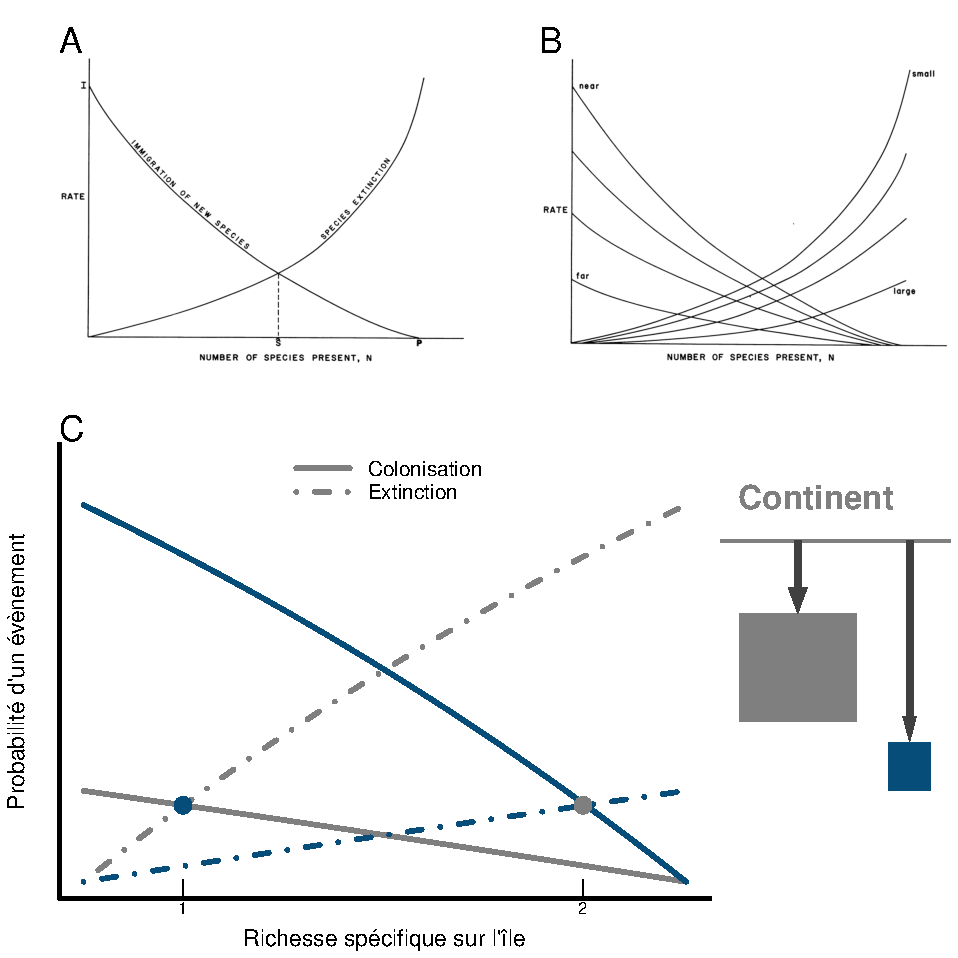
\includegraphics{fig/fig1.pdf}
\caption{\textbf{La Théorie de la biogéographie des Iles.} (A)
L'évolution des taux de colonisation et d'extinction est présentée pour
deux îles aux caractéristiques différentes. Les tailles relatives des
îles et les distances qui les séparent du continent sont schématisées à
droite du graphique, les couleurs associent les îles à leurs courbes
respectives. Le pool d'espèce régional (\(P\)) est constitué de 100
espèces, les taux de colonisation et d'extinction sont exprimés en terme
de probabilité d'évènement. Les points où colonisation et extinction
s'équilibrent sont marqué par les symboles en gris. (B) et (C) sont
respectivement les figures 4 et 5 extraites de l'article de 1963 de
MacArthur et Wilson qui livre essentiellemnt le même message illustré en
(A) (MacArthur and Wilson, 1963). La forme convexe des courbes de 1963
sont justifiées par des facteurs biologiques qui ne sont pas intégrés
dans l'équation \label{eqMW} qui donne une forne concave comme montré en
(A).\label{fig:figMW}}
\end{figure}

\subsubsection*{L'importance de la TIB dans des déveloopemnt théoriques
plus
récents}\label{limportance-de-la-tib-dans-des-duxe9veloopemnt-thuxe9oriques-plus-ruxe9cents}
\addcontentsline{toc}{subsubsection}{L'importance de la TIB dans des
déveloopemnt théoriques plus récents}

\subsubsection*{La théorie des
métapopulations}\label{la-thuxe9orie-des-muxe9tapopulations}
\addcontentsline{toc}{subsubsection}{La théorie des métapopulations}

Bien que ne représentant que cinq pourcents des teres émergeés, ce sont
bine l'observations des îles qui ont mené à une vision paradigmatique de
la biogéograaphie. IL est porbable que cela soit lié au caractère à leur
relative abondance, leur disparité, leur diversité, la relative
simplicité biologiques qu'on y trouve et très certianenment, comme je
l'ai évoqué précedemment, une lecture claire des flux de migration
(Simberloff, 1974). Cette dernière propriété est souvent absente pour
des populations continentales (et dès qu'on est en précence d'un
archipel). La théorie des métapopulations s'intéresse justement aux
populations reliées par des flux de migrations ({\textbf{???}}). C'est
Richard Levins qui a utilisé le premier le terme en 1970
({\textbf{???}}). En considérant des patch favorable, il détermine la
proportion de ces patchs occupés par une espèce donnée \(p\) en fonction
de ces capaicté de dispersion \(c\) et la probabilité d'extinction \(p\)
:

\begin{eqnarray}
\label{eqMW}
\frac{dp}{dt} = cp(1-p)-ep
\end{eqnarray}

Le taux de migration est proportionel à la proportion de pactch déjà
occupé. La théorie des metapopulations est aujourd'hui d'un certains
nombres de paradigmes (Leibold et al., 2004) et a montré sa pertinence
sur un certains nombre d'exemple concrets. Papillon Hanski 1998 / Hyloak
et bact.ir. /Matter 2092. et pour rebondire McPeek \& Brown (2000) have
investigated differences between competing damselfly species and finds
rather little difference among some species, leaving the neutral
paradigm as a potential explanation for high species diversity in this
groups of insect. opposition à la niche set de traits particuliers

\subsubsection*{La théorie neutre de la biogéographie et le débat
qu'elle
soulève}\label{la-thuxe9orie-neutre-de-la-bioguxe9ographie-et-le-duxe9bat-quelle-souluxe8ve}
\addcontentsline{toc}{subsubsection}{La théorie neutre de la
biogéographie et le débat qu'elle soulève}

La théorie neutre postule une équivalence écologique entre les individus
de différentes espèces et formalise l'idée d'un replacement perpétuel
d'un individu mort par un autre espèce morte par une autre, à la manière
de replacement par de nouveaux jeune arbres suite d'un chablis (Hubbell,
1999). Dans l'article fondateur de cette théorie, Stephen Hubbell décrit
um tirage aléatoire régit par l'abndance dans la communauté locale et la
colonisation d'un individu extérieur dont la probabilité dépend de son
abondance à l'échelle régionale. Cette théorie partage beaucoup de
charactéristiques avec la TIB, on y trouve un principe d'équivalence
décologique, une imbrication des échelles régionale et locales et un
accent sur le chacractère aléatoire des colonisaion mais aussi des
configuration locale des communautés. Comme le fait remaquer Hubbell en
2010 dans le chapitre qu'il écrit dans le livre mentionné plus haut,
\emph{The Theory of Island Biogeography Revisited}, la théorie neutre
place l'équivalence au niveau des individus et non plus au niveau des
espèces ({\textbf{???}}). Cette théorie a été très souvent attaqué (par
exemple (McGill and Collins, 2003)) pour le postulat déquivalence alors
même que la TIB ne l'a pas été (tout du moins pas au même niveau).
Néanmoins il n,est pas étonnat que cette idée est été poussé un cran
plus loin que dans la TIB pour justemnt voir ce que l'on peut dire en
faisant un minimu d'hypothèse sur la snglatiré

\begin{quote}
The symmetry assumption is equivalent to asking how many of the
properties of ecological communities are captured by the mean, ignoring
species differences.
\end{quote}

Pour les defenseurs de la théorie neutre, elle est aussi utile autant
vrai que fausse (Rosindell et al., 2012), c'est une jauge pur montrer si
les processus de processu domine ou pas (John et al., 2007). Pour
certains auteur, il s'agut d'un d.bat classique entre les r.alistes et
les inttrumentaliste, les uns d.taill. un bout de picture une image
globale flou mais les deux devrait beneficier (Wennekes et al., 2012)
surtout quand mathématqiuemnt il y a un pas entre les deux (Gravel et
al., 2006). Quoiqu'il en soit encore besoin de commaisance et essayer
plus loin ce que l'on peut particulariser notamment sur l'introduction
des interactions. Opposition à la niche mais que faire\ldots{}

\section*{Le rôle des interactions dans la distribution des
espèces}\label{le-ruxf4le-des-interactions-dans-la-distribution-des-espuxe8ces}
\addcontentsline{toc}{section}{Le rôle des interactions dans la
distribution des espèces}

Ma thèse a pour objectif de trouver des leviers pour comprendre comment
les interactions peuvent affecter les distributions d'espèce et de
comprendre où chercher les traces qu'elles pourraient laisser dans les
données d'occurrence des espèce. Comme je l'ai mentionnée auparavant
cette idée est très ancienne, je cite volontier Wallace qui écrit dès
l'introduction de son livre écrit :

\begin{quote}
« Both competition and predation appear now to be much more important in
biogeography than people had formely guesses (({\textbf{???}})) »
\end{quote}

Le problème auquel ce sont vraissemblablememnt est le caractère
singulier des relations qui unissent les être vivant et que dans la
recherche de point commun il n'est pas pu mettre au point une théorique
de la biogéographie des piles intégrant les interactions. Néanmoins, au
vie des développemnt de son dernier livre, on peut faire spéculer que
MacArthur ouvait réfléchir à une telle intégration (MacArthur, 1972).
C'est dans lobjectif d'aller vers une théorie plus intégrative mais
toute aussi élégante qyue j'ai mené ma thèse qui apporte quelques
pistes.

\subsection*{Importance des interactions dans la
distribution}\label{importance-des-interactions-dans-la-distribution}
\addcontentsline{toc}{subsection}{Importance des interactions dans la
distribution}

La théorie de la Biogéographie des îles (et il en va de même pour la
théorie neutre) est certes une théorie qui ne s'articule pas sur les
interactions et fais une forme d'équivalence écologique, les idées sont
clairemnent oser que localemnt les raisons profindes de l'extinciton
locale. La question que l'on peut alors se poser est de savoir si les
c'est si on peut aller plus loin qu'une simple enonciation des proncipes
tout en gardante une cohérence. Aiinsi i lsemble omportant que la
théorie de la Biog.éogrpahie doit intégrer des résultats précis en terme
de réseaux. Dans le premier chapitre j'ai poursuivi cette idées et est
montré qu'une approche communait centrés pouvat être prpoposé. Ne pas
considéere mdes espèces mais des aassembalges est une bonne échelle pour
aborder des problèmes des conséquences écologques des transients. Il est
aussi int.ressant que cela nous a fait glissé vers la compréhension des
résulats qu'om doit avoir dans les données de co-occurrene.

Accent sur les cascading effect est surtout un problème de l'instabiilté
({\textbf{???}}) Il ya aussi l'article perturbant de Säterberg et al.
(2013) qui montre que le fait qu'une espèce soit (ex. pêche) peut
conduirte à des extinctions d'autres espèces lié dans le réseau\ldots{}
Ces deux exemple montrent que les interactions peuvent mener à des
problèmes de prédicitons et donc porblèmes sur prévoir les services
ecosystémiques et c'est appuyer par Cahill et al. (2013) qui nous
indique en somme que le changemment des interactiosn biotiques ets la
voie privilégiée d'extintionciton dans un contexte de changement
climatique.

chap 2 geographical ecology

il prend comme exemple la compétition entre oiseau et un manque de
ressource pour une année partiuculièremnet sévère et que 19 and pas
assez pour voir et il conclut que

\begin{quote}
This is the main reason most evidence for competition is from
biogepgraphers.
\end{quote}

Distributiin des fauvettes \emph{Crateroscelis robusta} et \emph{C.runa}

Mais le p

\subsection*{Un problème d'échelle?}\label{un-probluxe8me-duxe9chelle}
\addcontentsline{toc}{subsection}{Un problème d'échelle?}

Oubli de ce facteur important de Ls SMDS\ldots{}

Les interactions intra et inter spécifiques constituent un facteur
rapidement pressenti comme responsable de la distribution spatiale des
espèces \cite{Levin1974}. L'interdépendance des espèces conditionne, en
effet, l'aspect favorable de l'environnement au sens large (biotique et
abiotique). Ainsi Godsoe \textit{et al.} 2012, mettent en équations le
caractère favorable de l'environnement pour une espèce donnée en terme
de probabilité de présence d'une autre espèce et de la nature de leur
interaction \cite{Godsoe2012}. De même, Holt et Barfield 2009 montrent
l'impact de la prédation sur la répartition d'espèces en compétition
\cite{Holt2009} insistant ainsi sur le rôle majeur des interactions.
Davis \textit{et al.} 1998 ont montrés que, pour trois drosophiles en
compétition, l'effet d'un parasitoïde n'est pas le même le long d'un
gradient selon que les espèces sont seules ou ensemble \cite{Davis1998}.
Récemment, des efforts ont été réalisés pour mettre en évidence
l'importance de l'interdépendance des espèces dans les données aux
larges échelles spatiales \cite{Gotelli2010}. On trouve actuellement
dans la littérature une grande motivation pour les intégrer dans les
modèles de distribution d'espèces \cite{Kissling2011, Guisan2011}. Des
efforts théoriques sont encore nécessaires pour arriver à de telles
approches. Néanmoins, rapprocher différents champs de l'écologie peut
s'avérer d'une utilité majeure. Jabot et Bascompte \cite{Jabot2012}
2012, ont d'ailleurs montré l'importance des interactions pour
comprendre la distribution des espèces en rapprochant écologie des
réseaux et un modèle de metacommunauté. De même Gravel \textit{et al.}
2011 \cite{Gravel2011b} introduise l'interdépendance proie-prédateur
dans le modèle classique de MacArthur et Wilson menant aux prémices
d'une théorie trophique de la biogéographie des îles.

L'ajout des interactions dans un modèle incluant l'environnement
abiotique interroge la relation que les deux processus entretiennent. Si
les espèces n'ont pas les mêmes performances dans différents milieux du
fait de leur physiologie, pour les mêmes espèces considérées, les
réseaux n'ont pas de raison d'être identiques d'un milieu à un autre.
C'est sur ce fait que Poisot \textit{et al.} 2012 ont proposé une mesure
de dissimilarité des réseaux \cite{Poisot2012}. Defossez \textit{et al.}
montrent que les interactions négatives entre l'hêtre commun
(\textit{Fagus Sylvaitca}) et les micro-organismes du sol diminuent avec
l'altitude \cite{Defossez2011}. Ainsi, les contraintes biotiques sont à
relier à l'environnement \cite{Brooker2006,Canham2006} et un modèle
intégratif doit donner un cadre cohérent à ces rétroactions entre
processus. Enfin, l'importance des interactions est à mettre en relation
avec l'échelle considérée \cite{Peterson2011}. Pour deux espèces en
interaction, plus l'échelle d'étude est large, moins les effets des
interactions locales sont susceptibles d'être capturés, le pouvoir
explicatif de la présence d'une espèce sur l'autre peut être alors
discutable \cite{Araujo2007}. Comprendre quels sont les processus à
prendre en compte aux différentes échelles spatio-temporelles et
comprendre comment le changement d'échelle affecte nous prédictions est
aussi un véritable challenge en biogéographie \cite{Martinez2012}.

\subsubsection{Un problème d'échelle
?}\label{un-probluxe8me-duxe9chelle-1}

Comment les varitions démogrpahiques interactions se propagent-t-elle à
travers les échelles spatiale.

\begin{quote}
However, it is argued that applying bio-climatic models at macro-scales,
where climatic influences on species distributions are shown to be
dominant, can minimize the impact of biotic interactions. Indeed, the
fact that a number of bioclimatic models have been highly successful at
simulating current species distributions at certain scales is in
fundamental disagreement with the proposition that species distributions
cannot be adequately defined by climatic factors alone. (Pearson and
Dawson, 2003)
\end{quote}

\begin{quote}
We will never be able to predict the future with accuracy, but we need a
strategy for using existing knowledge and bioclimatic modeling to
improve understanding of the likely effects of future climate on
biodiversity. (Araujo and Rahbek, 2006).
\end{quote}

Les ranges comme un fait (wallace chap 2) des espèces avec des larges
avec des grandes ranges Loddigésie admirable (\emph{Loddigesia
mirabilis}) seul collibris de son genre vs Lièvre variable (\emph{Lepus
timidus}) nomnbre d'espèce dans un genre vaire beaucoup =\textgreater{}
un autre indice de solution pas fructifiées\ldots{} Pithacia Monathus vs
Pithecia pythecia separé par une rivière Geographical Ecology
=\textgreater{} patterns in the distribution of spceies 2 espèces
proches des ranges très séparéed =\textgreater{} species Bonobo et
cChimpanzés

orblème étant que le signal n'est visible que si on a des données sur
20and.

Le problème

Parallèle entre information des traits sur le régime allimentaire et
l'information dans les ranegs est-ce cela qui conduit les ecologistes à
être des statisticuencs. et l'info dans l'ADN

\subsection{Faire un questionnement des intersections des ranges et des
règles}\label{faire-un-questionnement-des-intersections-des-ranges-et-des-ruxe8gles}

On a besoinde rule on reste descriptive il y a des relation
EH-Bioversité, SAR, Diversité-équilibre diversité fonctionnenemnt qui
sont partielelemnt reliées et des théries débat theories neutre theéor
de la niche Stein et al. (2014). Dans cette review Stein et al. (2014)
montre que vegetaiton est inportnates ce qui eimplique des
inbteractions. Théorie allométrique prometteuse en ce sens qu'elle loi
physiques. Différents concept autrour d'une même notion sur plusieurs
paradigme pour une même notion sur les metacommunity Leibold et al.
(2004) il peuvent co-exister mais faudrait les savoir ce qui fait qu'on
a pus l'un ou l'autr.

La puissance de la Biogéographie est aussi sont implications dans des
cas très concrets Cirtwill and Stouffer (2015) mais aussi ne puissance
exploratoire théoriques Gravel et al. (2011) Cazelles et al. (2015) des
îles l'idée des interactions à déjà montré ça pertinence sur plusieurs
exemples. Cirtwill and Stouffer (2015)

Les interactions quelles pourrait être leur conséquence à large échelle
?

\begin{quote}
(:154) ``Does the environment dictate the structure of the community, or
are the species a fairly random assemblage?
\end{quote}

Cette id.e aussi est données par

\begin{quote}
A few decades ago it as fashionable for ecologist to study communities
in the arctic on the grounds that these would be very simple communities
and hence easy to understand. Many excellent ecologists still follow
this belied, but there are others who feel that it may be easier to
understand the extremely complex communities. This sounds paradoxical:
How can a more complex communities by easier to understand? A possible
answer might be that complex community has has strong interactions among
species so that the lives of the separate species are less independent
than in a simple community. Where there is greater interdependence,
patterns may be more conspicuous."
\end{quote}

Information dans les distributions gecko australien généraliste
\emph{Heteronotia binoei} =\textgreater{}~alors peut être que ça marche
bien mais sur une espèce spécialiste ??

\begin{quote}
Generalist consumers should typically be weakly coupled to any one of
their prey populations because, when feeding on many different species,
they cannot be strongly coupled to any one of them Murdoch et al. (2002)
\end{quote}

Intégrations des contraintes biotiques et de la théorie à la recherche
de signaux de d'intéraction

Dans ma thèse j'ai oassé du temps à essayer de mettre au point un modèke
qui donnait de la substace aux idées de MacArthur et Wilson een etandant
le travai initié par Gravel et collègues pour aller plus loin dans la
compréhension des effets joints des interactions et des contraintes
abiotiques. C'est aussi ce qui m'a animé pour en mettre en place la
compréhesin dans les données de co-occurrence avant d'aller m'y
confronter frongalemnet. Ma dernière intergtaion a Été de trouver des
pistes pour allerr plus loin dans la théorie et explorer des pistes que
je n'avais pas encore dxplorer mais qui seront à court terme les
directions que je souhaite explorer.

Abondance des données Les atouts actuels de la biogéographie sont 1- une
quantité importante d'information relative aux présences d'espèces et au
climat et 2- des modèles corrélatifs puissants qui décrivent précisément
le lien entre l'espèce et son environnement abiotique. Le terme
abiotique peut prêter à confusion dans la mesure où les espèces
elles-mêmes peuvent modifier des variables dîtes abiotiques. Par
exemple, les végétaux peuvent avoir un grand impact sur les variables
abiotiques locales comme la température et l'humidité du sol
\cite{Breshears1998}. Certains auteurs font une distinction précise en
utilisant les termes de \textit{scenopoetiques} pour les variables
environnementales sur lesquels les espèces ne peuvent influer et de
\textit{dynamiquement liées} pour les autres \cite{Peterson2011}. Nous
occulterons volontairement ces-dernières, l'environnement abiotique dont
il est ici question n'est donc pas dynamiquement lié aux espèces.

Partir du development de la niche et des hypotheses clef comme
l'heterogeneité spatiale qui peut accroitre la biodiversité un exemple
c'est les ecoulemnents à petites faible echelles de l'hydrologie niche
hdrologique à fable échelles Letten et al. (2015) repartition
hydrologique les hypothèses sont qui explique celon les différentes
besoin des espèces (principes de la niche) que besoin différemtes me
répartition des espèces. Cette idées est

Mais une espèce généraliste autant que sécialiste Poisot et al. (2015)

A large espes répartition de la biodiversité on quantifie la différence
depuis les mesures classiques. Simpson, alpha gamma beta qui sont
étendues au réseau Poisot et al. (2012). Mais quand on chnage d'echelle
on arrive rarement à quelques choses de concluant pour l'integration des
interactions. Pourtant il ya des exemples convaicant comme celui de
Gitelli.

-- conclure en repartant sur l'exemple détaillé. Vespa aussi au Amérqieu
la densit. des traffic\ldots{} Multi couche de distrobution dans le cas
du frelon asiatique Villemant et al. ({\textbf{???}}) ont montrés que
superposition du genre \emph{Vespa} et notamment au niveau asiatique
énormément aisin l'inférence se fait sur des données qui comporte une
empreinte de condition et localemnt éteinte alors que possiblement
comtraite qui ne seront pas en France\ldots{} Essyer de faire des cartes
de risques plutôt que de constater après coup\ldots{} Après avoir fait
un retour sur plus de biologie je m,intergoge sur lesquelle dans la
suiste Dépasser les questionnemnet sur les espèces la contrainte il me
semble qu'une piste c'est aouverte avec des questions énergétique on se
rencontre qu'il y a des base én.ergétiqe dcommunet et que c'est ancrage
sit beaoup\ldots{}

\section*{annexes}\label{annexes}
\addcontentsline{toc}{section}{annexes}

\hypertarget{refs}{}
\hypertarget{ref-Allesina2012a}{}
Allesina, S., Tang, S., 2012. Stability criteria for complex ecosystems.
Nature 483, 205--208.
doi:\href{https://doi.org/10.1038/nature10832}{10.1038/nature10832}

\hypertarget{ref-TheArabidopsisGenomeInitiative2000}{}
Arabidopsis Genome Initiative, 2000. Analysis of the genome sequence of
the flowering plant Arabidopsis thaliana. Nature 408, 796--815.
doi:\href{https://doi.org/10.1038/35048692}{10.1038/35048692}

\hypertarget{ref-Araujo2006}{}
Araujo, M.B., Rahbek, C., 2006. How Does Climate Change Affect
Biodiversity? Science 313, 1396--1397.
doi:\href{https://doi.org/10.1126/science.1131758}{10.1126/science.1131758}

\hypertarget{ref-Balanya2006}{}
Balanyá, J., Oller, J.M., Huey, R.B., Gilchrist, G.W., Serra, L., 2006.
Global genetic change tracks global climate warming in Drosophila
subobscura. Science (New York, N.Y.) 313, 1773--5.
doi:\href{https://doi.org/10.1126/science.1131002}{10.1126/science.1131002}

\hypertarget{ref-Beck2012}{}
Beck, J., Ballesteros-Mejia, L., Buchmann, C.M., Dengler, J., Fritz,
S.A., Gruber, B., Hof, C., Jansen, F., Knapp, S., Kreft, H., Schneider,
A.-K., Winter, M., Dormann, C.F., 2012. What's on the horizon for
macroecology? Ecography 35, 001--011.
doi:\href{https://doi.org/10.1111/j.1600-0587.2012.07364.x}{10.1111/j.1600-0587.2012.07364.x}

\hypertarget{ref-Beck2014a}{}
Beck, J., Böller, M., Erhardt, A., Schwanghart, W., 2014. Spatial bias
in the GBIF database and its effect on modeling species' geographic
distributions. Ecological Informatics 19, 10--15.
doi:\href{https://doi.org/10.1016/j.ecoinf.2013.11.002}{10.1016/j.ecoinf.2013.11.002}

\hypertarget{ref-Bellard2012}{}
Bellard, C., Bertelsmeier, C., Leadley, P., Thuiller, W., Courchamp, F.,
2012. Impacts of climate change on the future of biodiversity. Ecology
letters 15, 365--377.
doi:\href{https://doi.org/10.1111/j.1461-0248.2011.01736.x}{10.1111/j.1461-0248.2011.01736.x}

\hypertarget{ref-Cahill2013}{}
Cahill, A.E., Aiello-Lammens, M.E., Fisher-Reid, M.C., Hua, X.,
Karanewsky, C.J., Ryu, H.Y., Sbeglia, G.C., Spagnolo, F., Waldron, J.B.,
Warsi, O., Wiens, J.J., 2013. How does climate change cause extinction?
Proceedings. Biological sciences / The Royal Society 280, 20121890.
doi:\href{https://doi.org/10.1098/rspb.2012.1890}{10.1098/rspb.2012.1890}

\hypertarget{ref-Cazelles2015b}{}
Cazelles, K., Mouquet, N., Mouillot, D., Gravel, D., 2015. On the
integration of biotic interaction and environmental constraints at the
biogeographical scale. Ecography n/a--n/a.
doi:\href{https://doi.org/10.1111/ecog.01714}{10.1111/ecog.01714}

\hypertarget{ref-Cirtwill2015}{}
Cirtwill, A.R., Stouffer, D.B., 2015. Knowledge of predator-prey
interactions improves predictions of immigration and extinction in
island biogeography. Global Ecology and Biogeography n/a--n/a.
doi:\href{https://doi.org/10.1111/geb.12332}{10.1111/geb.12332}

\hypertarget{ref-Connor1979}{}
Connor, E.F., Simberloff, D., 1979. The Assembly of Species Communities:
Chance or Competition? Ecology 60, 1132.
doi:\href{https://doi.org/10.2307/1936961}{10.2307/1936961}

\hypertarget{ref-Cook2002}{}
Cook, W.M., Lane, K.T., Foster, B.L., Holt, R.D., 2002. Island theory,
matrix effects and species richness patterns in habitat fragments.
Ecology Letters 5, 619--623.
doi:\href{https://doi.org/10.1046/j.1461-0248.2002.00366.x}{10.1046/j.1461-0248.2002.00366.x}

\hypertarget{ref-Desmet2004}{}
Desmet, P., Cowling, R., 2004. Using the species-area relationship to
set baseline targets for conservation. Ecology And Society 9, 1--39.

\hypertarget{ref-Diamond1975}{}
Diamond, J.M., 1975. Assembly of species communities, in: Cody, M.L.,
Diamond, J.M. (Eds.), Ecology and Evolution of Communities. Harvard
University Press, Cambridge, Massachusetts, USA., pp. 342--444.

\hypertarget{ref-Elith2006}{}
Elith, J., H. Graham, C., P. Anderson, R., Dudík, M., Ferrier, S.,
Guisan, A., J. Hijmans, R., Huettmann, F., R. Leathwick, J., Lehmann,
A., Li, J., G. Lohmann, L., A. Loiselle, B., Manion, G., Moritz, C.,
Nakamura, M., Nakazawa, Y., McC. M. Overton, J., Townsend Peterson, A.,
J. Phillips, S., Richardson, K., Scachetti-Pereira, R., E. Schapire, R.,
Soberón, J., Williams, S., S. Wisz, M., E. Zimmermann, N., 2006. Novel
methods improve prediction of species' distributions from occurrence
data. Ecography 29, 129--151.
doi:\href{https://doi.org/10.1111/j.2006.0906-7590.04596.x}{10.1111/j.2006.0906-7590.04596.x}

\hypertarget{ref-Elith2009a}{}
Elith, J., Leathwick, J.R., 2009. Species Distribution Models:
Ecological Explanation and Prediction Across Space and Time. Annual
Review of Ecology, Evolution, and Systematics 40, 677--697.
doi:\href{https://doi.org/10.1146/annurev.ecolsys.110308.120159}{10.1146/annurev.ecolsys.110308.120159}

\hypertarget{ref-Engelbrecht2007}{}
Engelbrecht, B.M.J., Comita, L.S., Condit, R., Kursar, T. a, Tyree,
M.T., Turner, B.L., Hubbell, S.P., 2007. Drought sensitivity shapes
species distribution patterns in tropical forests. Nature 447, 80--82.
doi:\href{https://doi.org/10.1038/nature05747}{10.1038/nature05747}

\hypertarget{ref-Finstermeier2013}{}
Finstermeier, K., Zinner, D., Brameier, M., Meyer, M., Kreuz, E.,
Hofreiter, M., Roos, C., 2013. A Mitogenomic Phylogeny of Living
Primates. PLoS ONE 8, 1--10.
doi:\href{https://doi.org/10.1371/journal.pone.0069504}{10.1371/journal.pone.0069504}

\hypertarget{ref-Gravel2011c}{}
Gravel, D., Bell, T., Barbera, C., Bouvier, T., Pommier, T., Venail, P.,
Mouquet, N., 2011. Experimental niche evolution alters the strength of
the diversity--productivity relationship. Nature 469, 89--92.
doi:\href{https://doi.org/10.1038/nature09592}{10.1038/nature09592}

\hypertarget{ref-Gravel2006a}{}
Gravel, D., Canham, C.D., Beaudet, M., Messier, C., 2006. Reconciling
niche and neutrality: the continuum hypothesis. Ecology letters 9,
399--409.
doi:\href{https://doi.org/10.1111/j.1461-0248.2006.00884.x}{10.1111/j.1461-0248.2006.00884.x}

\hypertarget{ref-Grinnell1917a}{}
Grinnell, J., 1917. The Niche-Relationships of the California Thrasher.
The Auk 34, 427--433.
doi:\href{https://doi.org/10.2307/4072271}{10.2307/4072271}

\hypertarget{ref-Hannah2013}{}
Hannah, L., Roehrdanz, P.R., Ikegami, M., Shepard, A.V., Shaw, M.R.,
Tabor, G., Zhi, L., Marquet, P.a., Hijmans, R.J., 2013. Climate change,
wine, and conservation. Proceedings of the National Academy of Sciences
110, 6907--6912.
doi:\href{https://doi.org/10.1073/pnas.1210127110}{10.1073/pnas.1210127110}

\hypertarget{ref-He2011}{}
He, F., Hubbell, S.P., 2011. Species-area relationships always
overestimate extinction rates from habitat loss. Nature 473, 368--71.
doi:\href{https://doi.org/10.1038/nature09985}{10.1038/nature09985}

\hypertarget{ref-Hijmans2005}{}
Hijmans, R.J., Cameron, S.E., Parra, J.L., Jones, P.G., Jarvis, A.,
2005. Very high resolution interpolated climate surfaces for global land
areas. International Journal of Climatology 25, 1965--1978.
doi:\href{https://doi.org/10.1002/joc.1276}{10.1002/joc.1276}

\hypertarget{ref-Hortal2011}{}
Hortal, J., Diniz-Filho, J.A.F., Bini, L.M., Rodríguez, M.Á., Baselga,
A., Nogués-Bravo, D., Rangel, T.F., Hawkins, B.A., Lobo, J.M., 2011. Ice
age climate, evolutionary constraints and diversity patterns of European
dung beetles. Ecology Letters 14, 741--748.
doi:\href{https://doi.org/10.1111/j.1461-0248.2011.01634.x}{10.1111/j.1461-0248.2011.01634.x}

\hypertarget{ref-Hubbell1999}{}
Hubbell, S.P., 1999. Light-Gap Disturbances, Recruitment Limitation, and
Tree Diversity in a Neotropical Forest. Science 283, 554--557.
doi:\href{https://doi.org/10.1126/science.283.5401.554}{10.1126/science.283.5401.554}

\hypertarget{ref-Jeschke2008}{}
Jeschke, J.M., Strayer, D.L., 2008. Usefulness of bioclimatic models for
studying climate change and invasive species. Annals of the New York
Academy of Sciences 1134, 1--24.
doi:\href{https://doi.org/10.1196/annals.1439.002}{10.1196/annals.1439.002}

\hypertarget{ref-John2007}{}
John, R., Dalling, J.W., Harms, K.E., Yavitt, J.B., Stallard, R.F.,
Mirabello, M., Hubbell, S.P., Valencia, R., Navarrete, H., Vallejo, M.,
Foster, R.B., 2007. Soil nutrients influence spatial distributions of
tropical tree species. Proceedings of the National Academy of Sciences
104, 864--869.
doi:\href{https://doi.org/10.1073/pnas.0604666104}{10.1073/pnas.0604666104}

\hypertarget{ref-Kearney2004}{}
Kearney, M., Porter, W.P., 2004. MAPPING THE FUNDAMENTAL NICHE:
PHYSIOLOGY, CLIMATE, AND THE DISTRIBUTION OF A NOCTURNAL LIZARD. Ecology
85, 3119--3131.
doi:\href{https://doi.org/10.1890/03-0820}{10.1890/03-0820}

\hypertarget{ref-Kefi2015}{}
Kéfi, S., Berlow, E.L., Wieters, E.A., Joppa, L.N., Wood, S.A., Brose,
U., Navarrete, S.A., 2015. Network structure beyond food webs: mapping
non-trophic and trophic interactions on Chilean rocky shores. Ecology
96, 291--303.
doi:\href{https://doi.org/10.1890/13-1424.1}{10.1890/13-1424.1}

\hypertarget{ref-Kefi2012}{}
Kéfi, S., Berlow, E.L., Wieters, E.A., Navarrete, S.A., Petchey, O.L.,
Wood, S.A., Boit, A., Joppa, L.N., Lafferty, K.D., Williams, R.J.,
Martinez, N.D., Menge, B.A., Blanchette, C.A., Iles, A.C., Brose, U.,
2012. More than a meal\ldots{} integrating non-feeding interactions into
food webs. Ecology Letters 15, 291--300.
doi:\href{https://doi.org/10.1111/j.1461-0248.2011.01732.x}{10.1111/j.1461-0248.2011.01732.x}

\hypertarget{ref-Koh2004}{}
Koh, L.P., 2004. Species Coextinctions and the Biodiversity Crisis.
Science 305, 1632--1634.
doi:\href{https://doi.org/10.1126/science.1101101}{10.1126/science.1101101}

\hypertarget{ref-Lavergne2010}{}
Lavergne, S., Mouquet, N., Thuiller, W., Ronce, O., 2010. Biodiversity
and Climate Change: Integrating Evolutionary and Ecological Responses of
Species and Communities. Annual Review of Ecology, Evolution, and
Systematics 41, 321--350.
doi:\href{https://doi.org/10.1146/annurev-ecolsys-102209-144628}{10.1146/annurev-ecolsys-102209-144628}

\hypertarget{ref-Leibold2004}{}
Leibold, M.a., Holyoak, M., Mouquet, N., Amarasekare, P., Chase, J.M.,
Hoopes, M.F., Holt, R.D., Shurin, J.B., Law, R., Tilman, D., Loreau, M.,
Gonzalez, a., 2004. The metacommunity concept: a framework for
multi-scale community ecology. Ecology Letters 7, 601--613.
doi:\href{https://doi.org/10.1111/j.1461-0248.2004.00608.x}{10.1111/j.1461-0248.2004.00608.x}

\hypertarget{ref-Letten2015}{}
Letten, A.D., Keith, D.a., Tozer, M.G., Hui, F.K., 2015. Fine-scale
hydrological niche differentiation through the lens of multi-species
co-occurrence models. Journal of Ecology 103, 1264--1275.
doi:\href{https://doi.org/10.1111/1365-2745.12428}{10.1111/1365-2745.12428}

\hypertarget{ref-Lomolino2000a}{}
Lomolino, M., 2000. Ecology's most general, yet protean pattern : the
species area relationship. Journal of Biogeography 27, 17--26.

\hypertarget{ref-Lomolino2000}{}
Lomolino, M.V., 2000. A call for a new paradigm of island biogeography.
Global Ecology and Biogeography 9, 1--6.
doi:\href{https://doi.org/10.1046/j.1365-2699.2000.00185.x}{10.1046/j.1365-2699.2000.00185.x}

\hypertarget{ref-Lomolino2009}{}
Lomolino, M.V., Brown, J.H., 2009. The reticulating phylogeny of island
biogeography theory. Q. Rev. Biol. 84, 357--390.
doi:\href{https://doi.org/10.1017/CBO9781107415324.004}{10.1017/CBO9781107415324.004}

\hypertarget{ref-Losos2010}{}
Losos, J.B., Ricklefs, R.E., 2010. The Theory of Island Biogeography
Revisited. Princeton University Press, Princeton, NJ.

\hypertarget{ref-macarthur1972geographical}{}
MacArthur, R.H., 1972. Geographical Ecology: Patterns in the
Distribution of Species, Biology / {[}princeton university press{]}.
Princeton University Press.

\hypertarget{ref-MacArthur1967}{}
MacArthur, R.H., Wilson, E.O., 1967. Theory of Island Biogeography,
Princeton landmarks in biology. Princeton University Press, Princeton,
NJ.

\hypertarget{ref-MacArthur1963}{}
MacArthur, R.H., Wilson, E.O., 1963. An equilibrium theory of insular
zoogeography. Evolution 17, 373--387.

\hypertarget{ref-May2004}{}
May, R.M., 2004. Uses and abuses of mathematics in biology. Science (New
York, N.Y.) 303, 790--3.
doi:\href{https://doi.org/10.1126/science.1094442}{10.1126/science.1094442}

\hypertarget{ref-May1973}{}
May, R.M., 1973. Stability and complexity in model ecosystems.
Monographs in population biology 6, 1--235.
doi:\href{https://doi.org/10.1109/TSMC.1978.4309856}{10.1109/TSMC.1978.4309856}

\hypertarget{ref-mccann2011food}{}
McCann, K.S., 2011. Food Webs, Monographs in population biology.
Princeton University Press.

\hypertarget{ref-McCann2000}{}
McCann, K.S., 2000. The diversity-stability debate. Nature 405, 228--33.
doi:\href{https://doi.org/10.1038/35012234}{10.1038/35012234}

\hypertarget{ref-McGill2003}{}
McGill, B., Collins, C., 2003. A unified theory for macroecology based
on spatial patterns of abundance. Evolutionary Ecology Research 5,
469--492.
doi:\href{https://doi.org/10.1038/nature01569.1.}{10.1038/nature01569.1.}

\hypertarget{ref-Murdoch2002}{}
Murdoch, W.W., Kendall, B.E., Nisbet, R.M., Briggs, C.J., McCauley, E.,
Bolser, R., 2002. Single-species models for many-species food webs.
Nature 417, 541--543.
doi:\href{https://doi.org/10.1038/417541a}{10.1038/417541a}

\hypertarget{ref-Neigel2003}{}
Neigel, J., 2003. Species-area relatioships and marine conservation.
Ecological Applications 13, 138--145.
doi:\href{https://doi.org/10.1890/1051-0761(2003)013\%5B0138:SARAMC\%5D2.0.CO;2}{10.1890/1051-0761(2003)013{[}0138:SARAMC{]}2.0.CO;2}

\hypertarget{ref-Pearson2003}{}
Pearson, R.G., Dawson, T.P., 2003. Predicting the impacts of climate
change on the distribution of species: are bioclimate envelope models
useful? Global Ecology and Biogeography 12, 361--371.
doi:\href{https://doi.org/10.1046/j.1466-822X.2003.00042.x}{10.1046/j.1466-822X.2003.00042.x}

\hypertarget{ref-Pelletier2007}{}
Pelletier, F., Clutton-Brock, T., Pemberton, J., Tuljapurkar, S.,
Coulson, T., 2007. The evolutionary demography of ecological change:
Linking trait variation and population growth. Science 315, 1571--1574.
doi:\href{https://doi.org/10.1126/science.1139024}{10.1126/science.1139024}

\hypertarget{ref-Pelletier2009}{}
Pelletier, F., Garant, D., Hendry, a P., 2009. Eco-evolutionary
dynamics. Philosophical transactions of the Royal Society of London.
Series B, Biological sciences 364, 1483--9.
doi:\href{https://doi.org/10.1098/rstb.2009.0027}{10.1098/rstb.2009.0027}

\hypertarget{ref-Poisot2012}{}
Poisot, T., Canard, E., Mouillot, D., Mouquet, N., Gravel, D., Jordan,
F., 2012. The dissimilarity of species interaction networks. Ecology
letters 15, 1353--61.
doi:\href{https://doi.org/10.1111/ele.12002}{10.1111/ele.12002}

\hypertarget{ref-Poisot2015c}{}
Poisot, T., Kéfi, S., Morand, S., Stanko, M., Marquet, P.A., Hochberg,
M.E., 2015. A continuum of specialists and generalists in empirical
communities. PLoS ONE 10, 1--12.
doi:\href{https://doi.org/10.1371/journal.pone.0114674}{10.1371/journal.pone.0114674}

\hypertarget{ref-Post2009}{}
Post, D.M., Palkovacs, E.P., 2009. Eco-evolutionary feedbacks in
community and ecosystem ecology: interactions between the ecological
theatre and the evolutionary play. Philosophical transactions of the
Royal Society of London. Series B, Biological sciences 364, 1629--40.
doi:\href{https://doi.org/10.1098/rstb.2009.0012}{10.1098/rstb.2009.0012}

\hypertarget{ref-Rcoreteam2015}{}
R Core Team, 2015. R: A Language and Environment for Statistical
Computing.

\hypertarget{ref-Razafindratsima2013}{}
Razafindratsima, O.H., Mehtani, S., Dunham, A.E., 2013. Extinctions,
traits and phylogenetic community structure: Insights from primate
assemblages in Madagascar. Ecography 36, 047--056.
doi:\href{https://doi.org/10.1111/j.1600-0587.2011.07409.x}{10.1111/j.1600-0587.2011.07409.x}

\hypertarget{ref-Ricklefs1987}{}
Ricklefs, R.E., 1987. Community diversity: relative roles of local and
regional processes. Science 235, 167--171.
doi:\href{https://doi.org/10.1126/science.235.4785.167}{10.1126/science.235.4785.167}

\hypertarget{ref-Robinet2016}{}
Robinet, C., Suppo, C., Darrouzet, E., 2016. Rapid spread of the
invasive yellow-legged hornet in France: the role of human-mediated
dispersal and the effects of control measures. Journal of Applied
Ecology.
doi:\href{https://doi.org/10.1111/1365-2664.12724}{10.1111/1365-2664.12724}

\hypertarget{ref-Rosindell2012}{}
Rosindell, J., Hubbell, S.P., He, F., Harmon, L.J., Etienne, R.S., 2012.
The case for ecological neutral theory. Trends in Ecology and Evolution
27, 203--208.
doi:\href{https://doi.org/10.1016/j.tree.2012.01.004}{10.1016/j.tree.2012.01.004}

\hypertarget{ref-Saterberg2013}{}
Säterberg, T., Sellman, S., Ebenman, B., 2013. High frequency of
functional extinctions in ecological networks. Nature 499, 468--70.
doi:\href{https://doi.org/10.1038/nature12277}{10.1038/nature12277}

\hypertarget{ref-Schoener2011a}{}
Schoener, T.W., 2011a. The Newest Synthesis : Understanding Ecological
Dynamics. Science 331, 426--429.
doi:\href{https://doi.org/10.1126/science.1193954}{10.1126/science.1193954}

\hypertarget{ref-Schoener2011}{}
Schoener, T.W., 2011b. The newest synthesis: understanding the interplay
of evolutionary and ecological dynamics. Science (New York, N.Y.) 331,
426--9.
doi:\href{https://doi.org/10.1126/science.1193954}{10.1126/science.1193954}

\hypertarget{ref-Sexton2009}{}
Sexton, J.P., McIntyre, P.J., Angert, A.L., Rice, K.J., 2009. Evolution
and Ecology of Species Range Limits. Annual Review of Ecology,
Evolution, and Systematics 40, 415--436.
doi:\href{https://doi.org/10.1146/annurev.ecolsys.110308.120317}{10.1146/annurev.ecolsys.110308.120317}

\hypertarget{ref-Simberloff1974a}{}
Simberloff, D.S., 1974. Equilibrium Theory of Island Biogeography and
Ecology. Annual Review of Ecology and Systematics 5, 161--182.
doi:\href{https://doi.org/10.1146/annurev.es.05.110174.001113}{10.1146/annurev.es.05.110174.001113}

\hypertarget{ref-Simberloff1969}{}
Simberloff, D.S., Wilson, E.O., 1969. Experimental Zoogeography of
Islands: The Colonization of Empty Islands. Ecology 50, 278--296.
doi:\href{https://doi.org/10.2307/1934856}{10.2307/1934856}

\hypertarget{ref-Simberloff1969a}{}
Simberloff, D.S., Wilson, E.O., 1969. Experimental zoogeography of
islands: a model for insular colonization. Ecology 50, 296--314.
doi:\href{https://doi.org/10.2307/1934856}{10.2307/1934856}

\hypertarget{ref-Springer2015}{}
Springer, A., Swann, D., Crimmins, M., 2015. Climate change impacts on
high elevation saguaro range expansion. Journal of Arid Environments
116, 57--62.
doi:\href{https://doi.org/10.1016/j.jaridenv.2015.02.004}{10.1016/j.jaridenv.2015.02.004}

\hypertarget{ref-Stein2014}{}
Stein, A., Gerstner, K., Kreft, H., 2014. Environmental heterogeneity as
a universal driver of species richness across taxa, biomes and spatial
scales. Ecology Letters n/a--n/a.
doi:\href{https://doi.org/10.1111/ele.12277}{10.1111/ele.12277}

\hypertarget{ref-Tao2010}{}
Tao, T., Vu, V., Krishnapur, M., 2010. Random matrices: Universality of
ESDs and the circular law. The Annals of Probability 38, 2023--2065.
doi:\href{https://doi.org/10.1214/10-AOP534}{10.1214/10-AOP534}

\hypertarget{ref-Thuiller2013}{}
Thuiller, W., Münkemüller, T., Lavergne, S., Mouillot, D., Mouquet, N.,
Schiffers, K., Gravel, D., 2013. A road map for integrating
eco-evolutionary processes into biodiversity models. Ecology Letters 16,
94--105. doi:\href{https://doi.org/10.1111/ele.12104}{10.1111/ele.12104}

\hypertarget{ref-Tingley2009}{}
Tingley, M.W., Monahan, W.B., Beissinger, S.R., Moritz, C., 2009. Birds
track their Grinnellian niche through a century of climate change.
Proceedings of the National Academy of Sciences of the United States of
America 106 Suppl, 19637--43.
doi:\href{https://doi.org/10.1073/pnas.0901562106}{10.1073/pnas.0901562106}

\hypertarget{ref-Vanbergen2013}{}
Vanbergen, A.J., 2013. Threats to an ecosystem service: Pressures on
pollinators. Frontiers in Ecology and the Environment 11, 251--259.
doi:\href{https://doi.org/10.1890/120126}{10.1890/120126}

\hypertarget{ref-Villemant2011}{}
Villemant, C., Barbet-Massin, M., Perrard, A., Muller, F., Gargominy,
O., Jiguet, F., Rome, Q., 2011. Predicting the invasion risk by the
alien bee-hawking Yellow-legged hornet Vespa velutina nigrithorax across
Europe and other continents with niche models. Biological Conservation
144, 2142--2150.
doi:\href{https://doi.org/10.1016/j.biocon.2011.04.009}{10.1016/j.biocon.2011.04.009}

\hypertarget{ref-Villemant2006}{}
Villemant, C., Haxaire, J., Streito, J., 2006. Premier bilan de
l'invasion de Vespa velutina Lepeletier en France (Hymenoptera,
Vespidae). Bulletin de la Société entomologique de France 111, 535--538.

\hypertarget{ref-Waldrop2016}{}
Waldrop, M.M., 2016. The hundred-year quest for gravitational waves ---
in pictures. Nature.
doi:\href{https://doi.org/10.1038/nature.2016.19340}{10.1038/nature.2016.19340}

\hypertarget{ref-wallace1881island}{}
Wallace, A.R., 1881. Island Life: Or, The Phenomena and Causes of
Insular Faunas and Floras, Including a Revision and Attempted Solution
of the Problem of Geological Climates. Harper \& brothers.

\hypertarget{ref-Wallace1860}{}
Wallace, A.R., 1860. On the Zoological Geography of the Malay
Archipelago. Journal of the Proceedings of the Linnean Society of
London. Zoology 4, 172--184.
doi:\href{https://doi.org/10.1111/j.1096-3642.1860.tb00090.x}{10.1111/j.1096-3642.1860.tb00090.x}

\hypertarget{ref-Wallace1858}{}
Wallace, A.R., 1858. On the Tendency of Varieties to depart indefinitely
from the Original Type. Proceedings of the Linnean Society Of London 3,
53--62.

\hypertarget{ref-Wennekes2012}{}
Wennekes, P.L., Rosindell, J., Etienne, R.S., 2012. The Neutral---Niche
Debate: A Philosophical Perspective. Acta Biotheoretica 60, 257--271.
doi:\href{https://doi.org/10.1007/s10441-012-9144-6}{10.1007/s10441-012-9144-6}

\hypertarget{ref-Yoshida2003}{}
Yoshida, T., Jones, L.E., Ellner, S.P., Fussmann, G.F., Hairston, N.G.,
2003. Rapid evolution drives ecological dynamics in a predator-prey
system. Nature 424, 303--6.
doi:\href{https://doi.org/10.1038/nature01767}{10.1038/nature01767}
